%% LyX 2.0.2 created this file.  For more info, see http://www.lyx.org/.
%% Do not edit unless you really know what you are doing.
\documentclass[ngerman,twoside, openright, cleardoubleempty]{scrreprt}
\usepackage{mathptmx}
\usepackage{helvet}
\usepackage{courier}
\renewcommand{\familydefault}{\rmdefault}
\usepackage[T1]{fontenc}
\usepackage[utf8]{inputenc}
\usepackage{minibox}
\usepackage{fancyhdr}
\pagestyle{fancy}
\setcounter{secnumdepth}{3}
\setlength{\parskip}{\medskipamount}
\setlength{\parindent}{0pt}
\usepackage{babel}
\usepackage{varioref}
\usepackage{url}
\usepackage{amsmath}
\usepackage{amssymb}
\usepackage{graphicx}
\usepackage[authoryear]{natbib}
\usepackage{nomencl}
\usepackage{amsfonts}
\usepackage{amsmath}
\usepackage{float}
\usepackage{appendix}
\usepackage{listings}
\usepackage[]{algorithm2e}
\RestyleAlgo{boxruled}


\renewcommand{\appendixpagename}{\appendixname}
\renewcommand{\appendixtocname}{\appendixname}

% the following is useful when we have the old nomencl.sty package
\providecommand{\printnomenclature}{\printglossary}
\providecommand{\makenomenclature}{\makeglossary}
\makenomenclature
\usepackage[unicode=true,pdfusetitle,
 bookmarks=true,bookmarksnumbered=true,bookmarksopen=true,bookmarksopenlevel=1,
 breaklinks=false,pdfborder={0 0 0},backref=page,colorlinks=false]
 {hyperref}

\makeatletter



%%%%%%%%%%%%%%%%%%%%%%%%%%%%%% User specified LaTeX commands.
\usepackage{a4wide}

%Mit diesem Paket lassen sich eigene farben definieren
\usepackage{color} 
\definecolor{lgrau}{rgb}{0.655, 0.659, 0.667} % Lemoine-Grau
\definecolor{lblau}{rgb}{0, 0.173, 0.322} % Lemoine-Blau

%Gesamtzahl der seiten aufrufbar mit \ref{TotPages}
\usepackage{totpages} %Gesamtzahl der seiten aufrufbar mit \ref{TotPages}

\usepackage{ifpdf} % part of the hyperref bundle
\ifpdf % if pdflatex is used

 % set fonts for nicer pdf view
 \IfFileExists{lmodern.sty}
  {\usepackage{lmodern}}{}

\fi % end if pdflatex is used

%Formatierung des Quellenverezichnis bei der Formatierung mit Name und Jahr
%Bei anderen Bibstyle-Dateien kann es notwendig sein diesen Abschnitt auszukommentieren.
\makeatletter
\renewcommand\@makefntext[1]{%
   \setlength{\hangindent}{1.3em}
   \noindent
   \hb@xt@\hangindent{%
      \hss\@textsuperscript{\normalfont\@thefnmark}\hspace{.5em}}#1}
\makeatother
%\renewcommand{\@cite}[2]{-{#1}-}
%\setlength{\bibhang}{7mm}
%>>> Ende Formatierung Quellebverzeichnis

%Besserer Zeilenumbruch von URLs
\usepackage{url}

\usepackage{ifpdf} % part of the hyperref bundle
\ifpdf % if pdflatex is used

 % set fonts for nicer pdf view
 \IfFileExists{lmodern.sty}
  {\usepackage{lmodern}}{}

\fi % end if pdflatex is used


%>>Formatierung der Verweise entweder Zeile 1 und/oder 2 & 3 mssen auskommentiert werden.
%\usepackage{hyperref}




% that links to image floats jumps
% to the beginning of the float and 
% not to its caption
\usepackage[figure]{hypcap}

%Abkürzungsverzeichnis
\def\nompreamble{\addcontentsline{toc}{chapter}{\nomname}\markboth{\nomname}{\nomname}}
\renewcommand{\nomname}{Abk\"urzungen und Akronyme}
\renewcommand{\nomlabel}[1]{\hspace{5em}#1\hfil}
\makenomenclature

%%%Beginn - Definition der Kopf- und Fußzeile
%%Seiten mit neuem Kapitel (plain) werden getrennt formatiert
\fancypagestyle{plain}{%
\fancyhf{}%
\fancyhead[RO, LE]{\textcolor{lgrau}{\textsf{\textbf{ \small \leftmark}}}}
\fancyhead[LO, RE]{\textcolor{lgrau}{\textsf{\textbf{ \small Modellierung von Niederspannungsnetzen}}}}

\fancyfoot[CO, CE]{\textcolor{lgrau}{\footnotesize \today}}
\fancyfoot[RO, LE]{\textcolor{lgrau}{\footnotesize Seite \thepage /\pageref{TotPages}}}
}
%%Alle anderen Seiten werden hier definiert (das kann aber auch mit der Def. oben identisch sein)
\fancyhf{}
\fancyhead[RO, LE]{\textcolor{lgrau}{\textsf{\textbf{ \small \leftmark}}}}
\fancyhead[LO, RE]{\textcolor{lgrau}{\textsf{\textbf{ \small Modellierung von Niederspannungsnetzen}}}}

\fancyfoot[CO, CE]{\textcolor{lgrau}{\footnotesize \today}}
\fancyfoot[RO, LE]{\textcolor{lgrau}{\footnotesize Seite \thepage /\pageref{TotPages}}}

%%keine Linie
\renewcommand{\headrulewidth}{0pt}
%%Nur Kapitelname ohne Nummer
\renewcommand{\chaptermark}[1]{\markboth{#1}{}}
%%%Ende - Definition der Kopf- und Fußzeile


%% Umdefinition der Bildunterschriften in Koma-skript
\setkomafont{captionlabel}{\sffamily\upshape\bfseries}
\setcapindent{0em}
\renewcommand*{\capfont}{\slshape\small}
\setcapwidth[l]{\textwidth}

\usepackage{pdfpages}

% Prüfung auf benötigte LaTeXPakete
\usepackage{ifthen}

% Die Seiten des Inhaltsverzeichnisses werden römisch numeriert,
% ein PDF-Lesezeichen für das Inhaltsverzeichnis wird hinzugefügt
%\let\myTOC\tableofcontents
%\renewcommand\tableofcontents{\frontmatter
%  \pdfbookmark[1]{\contentsname}{}
%  \myTOC
%  \mainmatter }

  %\bibstyle@natdin

   % Einzug der Belege nach der Einordnungsmarke
   %\setlength{\bibhang}{7mm}

\makeatother

\begin{document}

\subject{\vspace{-40mm}
Wissenschaftliche Arbeit\\
 zur Erlangung des Grades eines Master of Science\\
 an der Friedrich-Schiller-Universität Jena\vspace{15mm}
}


\title{Modellierung deutscher Niederspannungsverteilnetze auf Grundlage von OpenStreetMap-Daten}


\subtitle{\vspace{20mm}
}


\author{\textsc{\huge Jonas Gütter}\\
{\large Matrikel-Nummer: 152127}}


\date{\today}


\publishers{\noindent %
\begin{minipage}[t]{0.4\columnwidth}%
\noindent \begin{flushleft}
\hfill{}
\includegraphics[width=0.65\columnwidth]{bilder/Logo_FSU}\\
\vspace{6mm}

\par\end{flushleft}

\end{minipage}\hfill{}%
\begin{minipage}[t]{0.51\columnwidth}%
\noindent \begin{flushleft}
Friedrich-Schiller-Universität Jena\\
Institut für Geographie\\
Lehrstuhl für Geoinformatik\\
\medskip{}
Erstprüfer:\\
Dr. Jannes Münchow\\
\medskip{}
Zweitprüfer: \\
Prof. Alexander Brenning
\par\end{flushleft}%
\end{minipage}\vspace{-20mm}
}

\maketitle
\newpage{}

\thispagestyle{empty}

\begin{minipage}[c][1\totalheight][t]{1\columnwidth}%
\vspace{40em}
Ich versichere an Eides statt durch meine eigene Unterschrift, dass
ich die nachstehende Arbeit selbständig und ohne fremde Hilfe angefertigt
und alle Stellen, die wörtlich oder annähernd wörtlich aus Veröffentlichungen
genommen sind, als solche kenntlich gemacht habe. Die Versicherung
bezieht sich auch auf in der Arbeit gelieferte Zeichnungen, Skizzen,
bildliche Darstellungen und dergleichen.

\vspace{3em}
Jena, \today

\vspace{5em}
Jonas Gütter, \\
Matr.-Nr.: 152127%
\end{minipage}

\begin{minipage}[t]{1\columnwidth}%
\hyphenation{So-wjet-un-ion Stau-beck-en}%
\end{minipage}
\begin{abstract}

Die vorliegende Arbeit befasst sich mit der Erzeugung künstlicher Niederspannungsnetze in Deutschland, die etwa für Kostenschätzungen anstelle von realen Netzen betrachtet werden können, wenn Daten zu tatsächlichen Netzen nicht zur Verfügung stehen. Diese Aufgabe ist in zwei Bereiche unterteilt, zum einen die Erzeugung künstlicher Leitungsdaten und zum anderen die Erzeugung künstlicher Transformatorstationen. Die Leitungen werden zunächst erzeugt, indem das Straßennetz aus OpenStreetMap als Vorlage verwendet wird. Für die Transformatorstationen werden mittels einer logistischen Regression Prediktorvariablen bestimmt, die mit dem Vorhandensein einer Transformatorstation korreliert sind. Auf Basis dieser Variablen wird dann eine vorher mit Durchschnittswerten berechnete Anzahl an Transformatoren durch einen graphentheoretischen Algorithmus auf dem Straßennetz verteilt.
Die Methode liefert gute Ergebnisse für die Anzahl der Transformatoren, deren Position weicht jedoch in den meisten Fällen stark von der wirklichen Lage ab. Für die Erzeugung der Leitungsdaten ist eine genaue Validierung noch ausstehend. Eine präzise Abbildung des Niederspannungsnetzes ist nicht möglich, die erzeugten Netze können jedoch als Modellnetze genutzt werden, um etwa großräumige Kostenschätzungen durchzuführen.\\

The present thesis deals with the generation of artificial low voltage networks in Germany which can be used instead of real networks in example for cost estimates in the case of real network data not being available. The task is split up in two parts, one of them being the generation of artificial power lines and the other being the generation of artificial substations. The lines are initially generated by using the street network from OpenStreetMap as a template. The generation of substations begins with identifying a set of predictor variables which are correlated to the existence of substations by conducting a logistic regression. Based on these predictor variables a previously calculated number of substations is placed on the street network with a graph-theoretical algorithm. While the method delivers good results for the number of substations, their positions deviate strongly from the real locations. An accurate validation for the generation of the power lines is still pending. It turns out thate a precise mapping of the low voltage network is not possible, though the generated networks can serve as model grids for conducting large-scale cost estimates.

\end{abstract}

\section*{Danksagung}

Während der gesamten Zeit des Schreibens meiner Master-Arbeit wurde ich ausführlich von Frau Editha Kötter am Reiner Lemoine Institut betreut und beraten. Ich danke ihr dafür herzlich, ebenso den übrigen Mitarbeitern des Reiner Lemoine Instituts für zahlreiche hilfreiche Ratschläge und die gute Arbeitsatmosphäre.

Herrn Dr. Jannes Münchow danke ich ebenfalls für Betreuung und Beratung, außerdem Herrn Prof. Alex Brenning für die Bereitstellung von Muster-Arbeiten zur Orientierung.

Vielen Dank auch an Herrn Dr. Pascal Lenzner und  Herrn Dr. Christian Komusiewicz für Information und Beratung zu Algorithmen in der Graphentheorie.



\tableofcontents{}%

\begingroup 

\chapter*{Abbildungen und Tabellen}

\addcontentsline{toc}{chapter}{Verzeichnis der Abbildungen und Tabellen}

\let\chapter=\section 

\let\addchap=\addsec 

\listoffigures 

\listoftables

\endgroup %



\chapter*{Begriffserklärungen}

\addcontentsline{toc}{chapter}{Begriffserklärungen}

\textbf{Ortsnetz:} Bei einem Ortsnetz handelt es sich um ein Niederspannungsnetz, das durch eine Ortsnetzstation aus dem darüber liegendem Mittelspannungsnetz gespeist wird. Innerhalb einer Ortschaft gibt es in der Regel mehrere Ortsnetze, jeder von einer Ortsnetzstation ausgehende Leitungsstrang wird als separates Ortsnetz bezeichnet.

\textbf{Ortsnetzstation:} Die Ortsnetzstation besteht aus einem oder mehreren Transformatoren, die vom Mittelspannungsnetz aus einen Niederspannungsstrang versorgen. Die Lage einer Ortsnetzstation im Bezug zu den versorgten Leitungen ist für elektrotechnische Betrachtungen von Bedeutung, da große Entfernungen zwischen Ortsnetzstation und Verbrauchern elektrotechnisch ungünstig sind und unter Umständen verstärkte Leitungen erfordern. Aus diesem Grund ist es wichtig, Ortsnetzstationen in die Erzeugung künstlicher Netzstrukturen miteinzubeziehen.

\textbf{Lastgebiet:} Ein Lastgebiet wird in der vorliegenden Arbeit als zusammenhängendes Areal verstanden, in dem flächendeckend Strom verbraucht wird, und auf dem darum ein Stromverteilnetz existieren muss. Lastgebiete können meist mit Ortschaften gleichgesetzt werden, in manchen Fällen handelt es sich auch um einzelne Gebäudegruppen wie etwa Bauernhöfe.

\markboth{Abkürzungen und Akronyme}{}

\settowidth{\nomlabelwidth}{DAISY}
\printnomenclature{}

\nomenclature{Abk.}{Abkürzung}\nomenclature{o.S.}{ohne Sinn}\nomenclature{DAISY}{Dynamisches Auskunfts- und Informationssystem}

\begin{minipage}[t]{1\columnwidth}%
\global\long\def\kwh#1{#1\,\textrm{kWh}}


\global\long\def\ms#1{#1\,\unitfrac{m}{s}}
%
\end{minipage}


\chapter{Einführung\label{chap:Einführung}}

Im Jahr 2010 wurde von der Bundesregierung beschlossen, den Anteil der erneuerbaren 
Energien an der deutschen Stromversorgung von damals 17 \% auf bis zu 80 \% im Jahr 2050 zu erhöhen. Inzwischen beträgt dieser Anteil etwa 30 \%. Der Umstieg auf erneuerbare Energien geht mit einer stark veränderten Beanspruchung der Stromnetze einher. Diese sind ursprünglich dafür ausgelegt worden, Strom von wenigen großen Erzeugern hin zu vielen kleinen Verbrauchern zu transportieren. Durch das Aufkommen der erneuerbaren Energien entsteht jedoch vielerorts die Situation, dass Strom von Privathaushalten ins Netz eingespeist wird, der Stromfluss kehrt sich also um. Mit dem weiteren Ausbau der Nutzung erneuerbarer Energien ist zu erwarten, dass in naher Zukunft an vielen Stellen die vorhandenen Netze nicht mehr ausreichen, die Stromversorgung unter den veränderten Bedingungen zu gewährleisten \citep{dena2010}. Vor allem die Niederspannungsnetze, die mit einem Längenanteil von rund 65\%  den größten Teil der Leitungen in Deutschland ausmachen, sind von diesem Problem betroffen, da die Einspeisung durch Privathaushalte hauptsächlich dort stattfindet.

Um die Auslegung der zukünftigen Netze möglichst effektiv planen zu können, ist es wichtig, die heute bestehenden Netze zu untersuchen, um Schwachstellen zu finden und Maßnahmen für deren Behebung entwickeln zu können. Aus diesem Grund wurde am Reiner Lemoine Institut das Projekt open\_eGo (open electricity grid optimization) ins Leben gerufen, in dessen Rahmen diese Arbeit erstellt wurde. Ziel des Projekts ist es, ein öffentlich zugängliches Netzplanungsinstrument zu schaffen, indem auf einer virtuellen Forschungsplattform Daten zu den deutschen Stromnetzen zur Verfügung gestellt werden, und diese Daten zur Erstellung verschiedener Szenarien genutzt werden können. Die vorliegende Arbeit ist dabei im Bereich der Datenbereitstellung angesiedelt und stellt eine Methode vor, mit der künstliche Netzdaten für den Bereich der Niederspannung generiert werden können.

Bei der Analyse von Stromnetzen in der Niederspannungsebene besteht eine große Schwierigkeit in der mangelhaften Datenlage. Die Verteilnetzbetreiber stellen Daten zu ihren Netzen oftmals nicht frei zur Verfügung oder haben diese Daten noch nicht digitalisiert. Ein frei zugänglicher, vollständiger Datensatz der deutschen Niederspannungsnetze existiert daher gegenwärtig nicht. Um trotzdem repräsentative Aussagen zur Lage der deutschen Niederspannungsnetze machen zu können, wurden verschiedene Methoden entwickelt, mit denen künstliche Netzstrukturen erzeugt werden, die den tatsächlichen Netzen möglichst ähneln. Meist werden dafür Strukturparameter der Siedlungsstruktur herangezogen, um typische Netze zu erstellen. Jedoch weisen alle diese Ansätze einen sehr starken Generalisierungsgrad auf, bei denen die individuellen Netzformen verloren gehen. In dieser Arbeit wird eine Methode vorgestellt, die künstliche Netzstrukturen generiert und sich dabei an den realen Netzformen orientiert, sodass die erzeugten Leitungsverläufe immer den Leitungsverläufen der realen Netze ähnlich sehen. Dazu werden Straßendaten aus OpenStreetMap verwendet.

Das Ziel dieser Arbeit besteht darin, künstliche Netzstrukturen unter Zuhilfenahme von Straßendaten aus OpenStreetMap zu erzeugen. Dahinter steht die Annahme, dass das Straßennetz eine große Ähnlichkeit mit dem Niederspannungsnetz aufweist, da Niederspannungskabel in der Regel entlang von Straßen verlegt sind. So kann für jede Siedlung eine individuelle Netzstruktur erzeugt werden, die auf dem Aussehen des realen Netzes beruht. Die Daten werden aus OpenstreetMap in eine PostgreSQL-Datenbank importiert und dort mittels PostgreSQL- und Python-Skripten weiter verarbeitet.

Im Kapitel "`Grundlagen"' werden die wesentlichen Begrifflichkeiten erläutert, die für das Verständnis der Arbeit von Bedeutung sind, sowie die gegenwärtige Literatur zum Thema der Arbeit vorgestellt. Das Kapitel "`Methoden und Daten"' behandelt die Prozesse, mit denen das künstliche Leitungsnetz angelegt und die Transformatorstandorte bestimmt wurden, sowie die dafür benötigten Eingangsdaten und die Validierungsvorgänge der beiden Datensätze. Im Kapitel "`Ergebnisse"' werden die entstandenen Datensätze und die Validierungsergebnisse beschrieben, die im Kapitel "`Diskussion"' kritisch untersucht und bewertet werden. Das Kapitel "`Fazit"' fasst schließlich die Erkenntnisse der Arbeit zusammen und gibt einen Ausblick auf die mögliche Richtung zukünftiger Forschungsarbeiten in diesem Bereich.
	
\chapter{Grundlagen\label{chap:Grundlagen} }

\section{Aufbau des deutschen Stromnetzes\label{sec:Aufbau des deutschen Stromnetzes}}

Für die Modellierung eines Stromnetzes ist es zunächst wichtig, zu wissen, aus welchen Komponenten sich ein solches Netz zusammensetzt. Nach \citet{Rumpel1989} besteht ein Stromnetz aus Kabeln, Freileitungen und Unterstationen, die demzufolge alle in der Modellierung berücksichtigt werden müssten. Unter Unterstation ist dabei eine Einrichtung zum Schalten, Umformen und Verteilen elektrischer Energie zu verstehen. Meist handelt es sich dabei um eine Transformatorstation, die die Aufgabe hat, zwischen verschiedenen Spannungsebenen zu wechseln. Im Niederspannungsbereich wird diese auch als Ortsnetzstation bezeichnet. Der Betrieb mehrerer Spannungsebenen ist aus dem folgenden Grund notwendig: Verbrauchergeräte benötigen eine bestimmte Spannung, um funktionieren zu können. Diese Spannung ist aber für den Transport des Stroms über weite Strecken nicht praktikabel, da dabei zu große Transportverluste auftreten würden. Transport elektrischer Energie über weite Strecken ist nur möglich, indem die Spannung erhöht und damit die Stromstärke verringert wird. Die Transportverluste werden dadurch verringert, da diese quadratisch mit der Stromstärke abnehmen. Nach zurückgelegtem Transport wird die Spannung wieder verringert und die Stromstärke erhöht, damit der Strom von den Verbrauchergeräten genutzt werden kann \citep{Pelte2010}.
Die Änderung der Spannungen wird mit Hilfe von Transformatoren bewerkstelligt. In Deutschland sind die Stromnetze, wie in Tabelle \ref{Tab_Spannungsebenen} dargestellt, in vier Spannungsebenen unterteilt: Die Höchstspannung mit 380 kV, die Hochspannung mit 110 kV, die Mittelspannung mit 10 oder 20 kV sowie die Niederspannung mit 0,23 oder 0,4 kV \citep{Heuck2013}. Die Abhängigkeiten der verschiedenen Spannungsebenen sind schematisch in Abbildung \ref{Abb_Spannungsebenen} dargestellt. Die vorliegende Arbeit behandelt ausschließlich die Ebene der Niederspannung, da eine Modellierung aller Spannungsebenen zugleich das Ausmaß einer Master-Arbeit übersteigen würde.

\begin{table}[h]

\noindent \begin{centering}
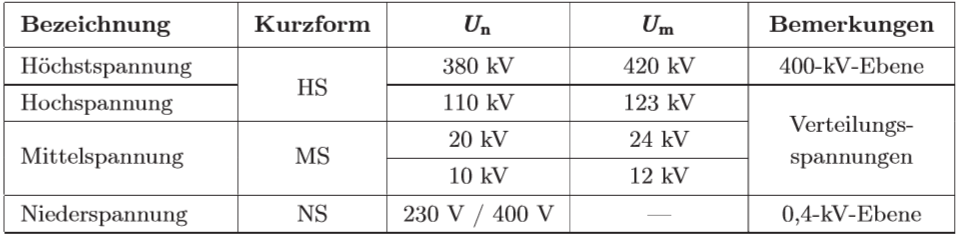
\includegraphics[keepaspectratio,width=\textwidth,height=\textheight]{bilder/Tabelle_Spannungsebenen}
\caption{übliche Spannungsebenen in Deutschland\label{Tab_Spannungsebenen}}
\par\end{centering}
\citep{Heuck2013}

\end{table}

\begin{figure} [t]

\noindent \begin{centering}
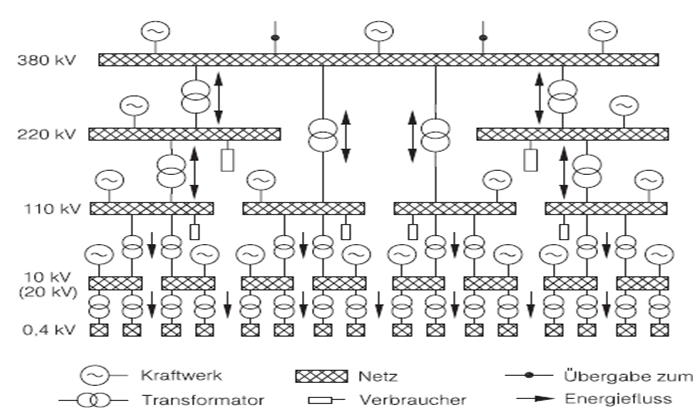
\includegraphics[keepaspectratio,width=0.75\textwidth,height=0.75\textheight]{bilder/Spannungsebenen}
\caption{Hierarchie der deutschen Stromnetze\label{Abb_Spannungsebenen}}
\par\end{centering}
\citep{Heuck2013}

\end{figure}

Planung und Betrieb der Stromnetze werden in Deutschland von privatwirtschaftlich organisierten Energieversorgungsunternehmen (EVU) vorgenommen \citep{Heuck2013}. Zurzeit gibt es über 800 EVU in Deutschland \citep{Statista2016}. Der größte Teil der Endverbraucher bezieht Strom aus den Niederspannungsnetzen, auch Ortsnetze genannt. Diese befinden sich am unteren Ende der Netzebenenhierarchie und werden durch Ortsnetzstationen von den übergeordneten Mittelspannungsnetzen versorgt. Ein Ortsnetz erstreckt sich meist über eine Fläche von weniger als einem Quadratkilometer \citep{Mohrmann2012} und kann sowohl durch Kabel als auch durch Freileitungen verlegt sein. Die Mehrzahl der deutschen Niederspannungsnetze ist allerdings kabelgeführt, Freileitungen spielen eher eine untergeordnete Rolle \citep{Kerber2008} und werden auch in Zukunft zunehmend durch Kabel ersetzt. Aus diesem Grund werden Freileitungen in den in Kapitel \ref{chap:Methoden und Daten} beschriebenen Methoden vernachlässigt. Niederspannungsnetze sind oftmals als Radial- oder Strahlennetze geführt \citep{Rumpel1989}, die sich dadurch auszeichnen, dass von einer einzelnen zentral gelegenen Ortsnetzstation die Leitungsstränge strahlenförmig nach außen abgehen, wie in Abbildung \ref{Netzformen} gezeigt. Ein Sonderfall der Strahlennetze bilden die Anschluss- oder Stummelnetze. Diese werden hauptsächlich in Innenstädten bei sehr großen Lastdichten eingesetzt und erstrecken sich nur über sehr kleine Gebiete. Bei einem Strahlennetz sind die einzelnen Leitungsstränge nicht miteinander verbunden. Manchmal gibt es jedoch offene Verbindungsstellen zwischen den Strängen, die bei Bedarf - zum Beispiel bei einer Störung im Netz - geschlossen werden können. Die so entstehende Netzform nennt man Ringnetz (siehe Abbildung \ref{Netzformen}). Eine weitere, hauptsächlich in städtischen Gebieten mit hoher Lastdichte vorkommende Netzform ist die des Maschennetzes. Bei diesem sind mehrere Ortsnetzstationen durch Leitungen miteinander verbunden, wie in Abbildung \ref{Netzformen} gezeigt. Aufgrund von Schwierigkeiten bei der Wiederinbetriebnahme solcher Netze nach Störungen werden jedoch seit den siebziger Jahren kaum noch Maschennetze neu geplant \citep{Heuck2013}. 

\begin{figure}

\noindent \begin{centering}
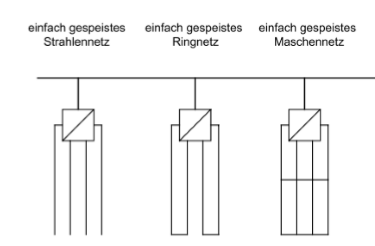
\includegraphics[keepaspectratio,width=\textwidth/2,height=\textheight/2]{bilder/Netzformen}
\caption{Übliche Netzformen von Stromverteilnetzen\label{Netzformen}}
\par\end{centering}
\citep{Scheffler2002}

\end{figure}


Nicht alle Verbraucher beziehen ihren Strom aus Niederspannungsnetzen. Industriebetriebe sind in manchen Fällen direkt an ein Mittelspannungsnetz angeschlossen, wenn deren Betriebsmittel einen entsprechenden Spannungsbedarf aufweisen. Mittelspannungsnetze werden über Umspannstationen aus den Hochspannungsnetzen gespeist und setzen sich sowohl aus Freileitungen als auch aus unterirdischen Kabeln zusammen, wobei in städtischen Gebieten fast ausschließlich Letztere verwendet werden. Mittelspannungsnetze sind oft in Form von Ringnetzen mit offenen Trennstellen aufgebaut, die im Betrieb als Strahlennetze fungieren. Maschennetze werden auf dieser Spannungsebene eher vermieden. Jede Ringleitung versorgt im Normalfall 5 bis 10 Ortsnetzstationen \citep{Heuck2013}.
Im Bereich der Hochspannung sind keine Verbraucher direkt an die Netze angeschlossen, vereinzelt findet dort bereits die Einspeisung aus Kraftwerken statt. Größtenteils werden die Hochspannungsnetze jedoch über Umspannwerke aus den darüber liegenden Höchstspannungsnetzen versorgt \citep{Heuck2013}. Diese verbinden den Großteil der Kraftwerke mit den Umspannwerken. Die Hoch- und Höchstspannungsnetze werden auch als Transport- oder Übertragungsnetze bezeichnet und sind hauptsächlich aus Freileitungen aufgebaut, unterirdische Kabel bilden eher die Ausnahme \citep{Zahoransky2010}. Die Übertragungsnetze in Deutschland werden von vier Gesellschaften betrieben: E.ON, Vattenfall Europe, RWE und EnBW. In Abbildung \ref{UENB_Bezirke} ist die regionale Aufteilung dieser Unternehmen auf das Bundesgebiet zu sehen.

\begin{figure}[t]

\noindent \begin{centering}
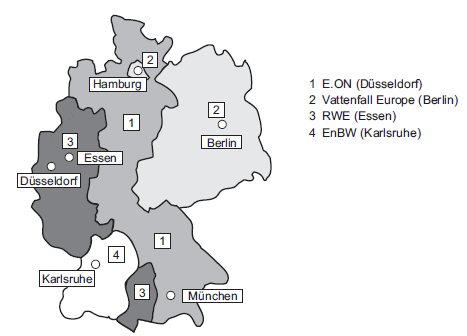
\includegraphics[keepaspectratio,width=\textwidth,height=\textheight]{bilder/UENB_Bezirke}
\caption{Übertragungsnetzgebiete in Deutschland\label{UENB_Bezirke}}
\par\end{centering}
\citep{Heuck2013}

\end{figure}

\section{Erzeugung künstlicher Netzstrukturen in der Niederspannung }

Zur Erzeugung künstlicher Netzstrukturen in der Niederspannung gibt es zahlreiche Arbeiten, da die Erhebung realer Netzdaten oftmals sehr aufwändig ist oder diese - im Falle der Neuplanung - noch gar nicht existieren. Vor allem die Arbeiten von Mohrmann et al., Scheffler und Kerber sind hierbei hervorzuheben, da diese grundlegende Methoden und Erkenntnisse für die Nachbildung von deutschen Niederspannungsnetzen beinhalten, auf denen auch Arbeiten anderer Autoren aufbauen \citep{Demirel2013, Gust2014, Lindner2016}.

Scheffler untersucht die zulässige Netzanschlussleistung von Photovoltaik-Anlagen in Wohngebieten. Er nennt die Siedlungsstruktur als bestimmenden Faktor für die Beschaffenheit von Netzen und nutzt eine Siedlungsklassifikation des Bundesamtes für Bauwesen und Raumordnung für deren Unterscheidung. für jeden Siedlungstyp erhebt er auf Basis von Netzplänen eines städtischen und eines regionalen Netzbetreibers die hauptsächlich vorkommenden Werte bestimmter Netzparameter. Mit Hilfe des Siedlungstyps und bestimmter Strukturparameter werden daraufhin durchschnittliche Netzparameter bestimmt. Diese Netzparameter sind für eine elektrotechnische Betrachtung nützlich, allerdings sind die dafür notwendigen Strukturparameter sowie der Siedlungstyp für eine große Anzahl einzelner Ortschaften, wie es in der vorliegenden Arbeit notwendig ist, nur schwer zu erheben. Die von Scheffler erhobenen typischen Netzparameter können jedoch für die Erzeugung künstlicher Netzstrukturen genutzt werden \citep{Scheffler2002}.

Kerber untersucht die	Aufnahmefähigkeit von Niederspannungsnetzen für Einspeisung aus Photovoltaik-Anlagen und erstellt für diesen Zweck Referenznetze. Er betrachtet dabei keine dicht besiedelten urbanen Regionen, da diese in der Regel sowohl eine niedrige PV-Einspeisung als auch stark ausgebaute Netze aufweisen und somit in diesen Gebieten nicht mit Problemen durch PV-Einspeisung zu rechnen ist. Stattdessen werden Land-, Dorf- und Vorstadtnetze betrachtet und anhand einer statistischen Untersuchung von 86 Netzen eine Reihe von Parametern bestimmt. Von diesen Parametern werden der mittlere Hausabstand, die Bemessungsleistung des Transformators und die verbraucherspezifische Transformatorleistung als am besten geeignet für die Trennung der betrachteten Netzklassen identifiziert. Auf Basis der ermittelten Parameter werden für jede der drei Netzklassen zwei charakteristische Referenznetze entwickelt, jeweils ein durchschnittliches und ein Extremwertnetz. Lokal unterschiedliche Gelände- und Bebauungsformen werden bei diesem Ansatz jedoch nicht berücksichtigt. Auch wird auf die Verteilung und den Standort der Transformatoren innerhalb eines Ortes nicht eingegangen \citep{Kerber2011}.

Mohrmann et al. erzeugen künstliche Netzstrukturen auf Basis von Mengengerüsten mit dem Ziel, Untersuchungen von Niederspannungsnetzen zu vereinfachen. Sie erheben Parameter anhand einer Analyse von 2700 Niederspannungsnetze mit vornehmlich ländlicher Prägung. für jeden der 5 Parameter werden drei bis sechs typische Ausprägungen angegeben. Aus den Kombinationen dieser Parameter können 810 unterschiedliche Netztopologien erzeugt werden. Von den bisher genannten Arbeiten weisen sie somit die größte Vielfalt in den Netzstrukturen auf. Die Mengengerüste, die zur Erzeugung dieser Netzstrukturen erforderlich sind, sind allerdings aufgrund der Datenlage schwer zu erstellen, auch geben die erzeugten Strukturen nicht notwendigerweise die Form der zugehörigen realen Netze wieder \citep{Kerber2011}.

Weitere Möglichkeiten der Modellierung sowie der Erzeugung synthetischer Netzstrukturen werden in den Arbeiten von Demirel, Lindner et al. und Schlömer et al. beschrieben. Demirel modelliert Niederspannungsnetze, indem er verschiedene elektrotechnische Randbedingungen wie z.B. die maximale Leitungslänge und die maximal übertragbare Leistung im Netzstrahl berechnet. Zur Berechnung dieser Werte ist allerdings Vorwissen zu bestimmten Eigenschaften des Netzes, wie z.B. der mittlere Hausabstand und die durchschnittliche Zahl an Wohneinheiten je Hausanschluss notwendig \citep{Demirel2013}. Lindner et al. stellen ein Verfahren zur Erzeugung künstlicher Niederspannungsnetze vor, bei dem sie insgesamt 31 elektrische sowie geographische Parameter aus einem Datensatz von 358 digitalisierten Niederspannungsnetzen ermitteln und diese Netze nach einer an \citet{Kerber2011} angelehnten Methodik klassifizieren. für jede Netzklasse werden typische Parameterausprägungen ermittelt, welche sodann für die Erzeugung von künstlichen Netzstrukturen verwendet werden. Diese werden abschließend darauf überprüft, ob die zulässigen Spannungsbänder sowie die Belastbarkeit der Betriebsmittel eingehalten sind \citep{Lindner2016}.
Schlömer et al. erzeugen ebenfalls synthetische Netzstrukturen in der Niederspannung, um verschiedene Möglichkeiten des Netzausbaus miteinander vergleichen zu können. Sie erzeugen einzelne synthetische Stränge durch Vereinfachungen, die nahe an beobachteten realen Netzen liegen, wie zum Beispiel die gleichmäßige Verteilung von Hausanschlüssen über den Netzstrang oder eine maximale Anzahl von 2 Kabelverteilerschränken pro Strang. Sie analysieren anschließend reale Netzstrukturen, indem diese in Einzelstränge zerlegt und diese Einzelstränge dann einer synthetischen Netzstruktur zugeordnet werden. Zum Schluss erfolgt eine Rekombination der Einzelstränge zurück zum Gesamtnetz \citep{Schloemer2014}. für Netze höherer Spannungsebenen in Amerika erzeugen Soltan et al. synthetische Netzstrukturen  mit dem Ziel, vollständige Netzdaten für die Forschung zur Verfügung stellen zu können, ohne das Sicherheitsrisiko der Veröffentlichung realer Netzdaten eingehen zu müssen. Die strukturellen und räumlichen Eigenschaften der realen Netze sollen folglich in den synthetischen Strukturen erhalten bleiben. Dafür werden bestimmte Parameter von den realen Netzen erhoben, die als Eingangsdaten für den Erzeugungsalgorithmus fungieren. Dieser verwendet ein Gauss'sches Mix-Modell, um die Knotenpunktdichte des Netzes zu schätzen und einen Datensatz von Knotenpunkten mit ähnlicher Dichte zu erzeugen. Mittels des Geographical Network Learner and Generator Algorithmus werden anschließend die Knotenpunkte untereinander verbunden, wobei versucht wird, eine maximale Konnektivität und Robustheit zu erreichen \citep{Soltan2015}.

Weiterhin existiert eine Reihe von Arbeiten zur Neuplanung elektrischer Netze, deren Methodik sich möglicherweise für die Modellierung bestehender Netze einsetzen lässt. Navarro et al. stellen eine solche Methodik vor, bei der das Straßennetz mitberücksichtigt wird. Das Planungsgebiet wird dabei aufgeteilt in kleinere Gebiete, sogenannte 'mini-zones'. Für diese Aufteilung werden drei verschiedene Methoden vorgestellt: Die erste besteht in der Erzeugung von Voronoi-Polygonen, die zweite nutzt die sogenannte Netzwerk-Rekombination, und die dritte verbindet schließlich beide Ansätze. Zur Anwendung empfohlen wird die Hybrid-Methode, in der beide Ansätze verwendet werden. Die Erzeugung der geplanten Netzstrukturen läuft so ab, dass in jeder 'mini-zone' ein Transformatorstandort festgelegt und seine Leistung anhand der zu versorgenden Verbraucher bestimmt wird. Von diesem Transformator ausgehend werden die Stromleitungen zu den Endverbrauchern erzeugt, die entlang des Straßennetzes verlaufen. Nach Erzeugung des Netzes werden die Kosten dieses Netzes abgeschätzt. Dieser Prozess wird mehrmals ausgeführt, wobei immer ein Transformator mehr als im vorherigen Schritt gesetzt wird. Der Prozess wird so oft wiederholt, bis die Kosten einer Iteration die der Vorgänger-Iteration übersteigen. Es wird dann angenommen, dass ein Kostenminimum bei der Vorgänger-Iteration erreicht ist und das entsprechende Netz als das optimale Netz betrachtet. für diese Methode müssen allerdings die Lage sowie der Stromverbrauch aller Endverbraucher bekannt sein \citep{Navarro2009a, Navarro2009b}. Eine Software zur Planung von elektrischen Netzen wird von Karpov et al. vorgestellt. Diese ist objekt-orientiert aufgebaut und unterstützt agentenbasierte Modellierung, wobei ein Agent eine Komponente des Modells darstellt. Die Modellierung des Netzes basiert auf folgenden Schritten:

\begin{itemize}
\item Bestimmung der Anzahl und des Typs von Stromerzeugern
\item Auswahl der Übertragungsleitungen
\item Untersuchung der Zuverlässigkeit und der Betriebsführung
\item Bestimmung der Prinzipien der Kontrollstrukturen
\end{itemize}

Die bei diesen Schritten zu treffenden Entscheidungen werden mit Hilfe mathematischer Gleichungen formalisiert. für den Zweck der vorliegenden Arbeit ist diese Software jedoch nicht geeignet, da hier keine Netze neu geplant, sondern vorhandene Netze abgebildet werden sollen \citep{Karpov2005}. Miguez et al. entwickeln einen Algorithmus zur Planung von Übertragungsnetzen in der Mittelspannung. Die Planung des Netzes wird von ihnen als Optimierungsproblem betrachtet: Eine Kostenfunktion wird aufgestellt, deren Minimum gefunden werden soll, indem ausgehend von einem Initialzustand solange einzelne Leitungen ersetzt werden, bis ein Kostenminimum erreicht ist. Miguez et al. gehen von radialen Netzstrukturen aus, sodass der Netzaufbau mit dem eines Niederspannungsnetzes vergleichbar ist. Allerdings werden die Lage der Endverbraucher sowie der Transformatoren als bekannt vorausgesetzt, was in der vorliegenden Arbeit nicht der Fall ist \citep{Miguez2002}.

Abschließend sei noch eine Arbeit von Schlömer et al. genannt, in der die Optimierung von Niederspannungsnetzen mithilfe von Methoden aus dem Forschungsfeld der Operations Research betrieben wird, bei dem es um die Planung und Optimierung von Unternehmensstandorten geht. Schlömer et al. übertragen dieses Prinzip auf potentielle Standorte von Ortsnetztransformatoren, denen Hausanschlüsse zugeordnet werden. Diese Aufgabe wird als Optimierungsproblem behandelt, bei dem eine Kostenfunktion minimiert werden soll. Zur Lösung dieses Problems wird der sogenannte Repeated Matching Algorithmus gewählt: Dieser ordnet wiederholt eine Gruppe von Hausanschlüssen einer Ortsnetzstation zu. Wenn die Kosten dadurch sinken, wird die Änderung übernommen, und die nächste Iteration begonnen. Es wird solange iteriert, bis ein Kostenminimum erreicht ist \citep{Schloemer2016}. 

\section{Das OpenStreetMap-Projekt}

Zur Modellierung des Niederspannungsnetzes werden Straßendaten aus OpenStreetMap verwendet.
Das OpenStreetMap-Projekt wurde 2004 gegründet und hat die Erzeugung eines Kartendatensatzes zum Ziel, der unter einer offenen Lizenz steht und der frei genutzt und editiert werden kann \citep{Haklay2008}. Neben Straßendaten sind auch vielfältige Daten zur Landnutzung, Landbedeckung und Siedlungsstruktur in der OpenStreetMap-Datenbank enthalten. Erhoben werden diese Daten durch eine große Zahl von Freiwilligen ohne spezielle kartographische Ausbildung. Initiativen wie das OpenStreetMap-Projekt, bei denen die Datengrundlage aus nutzergenerierten Geodaten besteht, werden unter dem Begriff Volunteered Geographic Information (VGI) zusammengefasst \citep{Goodchild2007}. Einer der Vorteile von VGI gegenüber kommerziellen Datenanbietern besteht darin, dass die Daten in der Regel kostenlos und unter einer freien Lizenz verfügbar sind. Außerdem beinhalten sie oft spezialisierte Informationen, deren Erhebung für kommerzielle Anbieter nicht wirtschaftlich wäre. Auf der anderen Seite ist die Erfassung der Datenqualität bei VGI-Projekten oftmals schwierig, da zahlreiche Nutzer nach unterschiedlichen Vorgehen Daten einarbeiten. Auch sind Informationen, für die spezielle Ausrüstung oder Expertenwissen benötigt wird, nur selten in VGI-Projekten zu finden, da die Datenerhebung meist von Freiwilligen ohne entsprechende Ausbildung durchgeführt wird. OpenStreetMap-Daten werden unter anderem bereits für 3D-Anwendungen \citep{Goetz2012}, im Katastrophenmanagement und vor allem zur Routenplanung eingesetzt.

Eine große Schwierigkeit bei der Verwendung von OpenStreetMap-Daten für wissenschaftliche Zwecke besteht in der Beurteilung der Datenqualität. Bei der großen Anzahl an zum Projekt beitragenden Personen liegt es auf der Hand, dass nicht überall mit der gleichen Vorgehensweise und Gründlichkeit gearbeitet wird. Auch hängt die Anzahl an Personen, die ein Gebiet bearbeiten, stark von der Lage des Gebiets ab. Das hat zur Folge, dass unter anderem Lagegenauigkeit, Attributgenauigkeit, Vollständigkeit und logische Konsistenz der OpenStreetMap-Daten stark variieren, je nachdem welche Region betrachtet wird. für die vorliegende Arbeit ist vor allem die Vollständigkeit der Straßendaten in Deutschland von Bedeutung, da bei mangelnder Vollständigkeit potentielle Stromleitungen übersehen werden könnten und bei stark schwankender Vollständigkeit zwischen Regionen starke Unterschiede in den resultierenden Stromnetzen entstehen würden. Untersuchungen zur Vollständigkeit von OpenStreetMap-Daten wurden bisher von Haklay in England und von Neis et al. in Deutschland angestellt.

Haklays Untersuchung basiert auf einem Vergleich von OpenStreetMap-Daten aus dem Jahr 2008 mit einer britischen amtlichen Landvermessungskarte und bezieht sich ausschließlich auf Straßen. für die Untersuchung der Vollständigkeit erstellt er ein 1km-Gitternetz über ganz England und bestimmt in jeder Gitterzelle den Unterschied zwischen der aufsummierten Straßenlänge aus OpenStreetMap und dem amtlichen Datensatz. Er kommt zu dem Ergebnis, dass die Gesamtlänge der betrachteten OpenStreetMap-Straßen nur 69\% der Gesamtlänge der Straßen aus dem amtlichen Datensatz ausmacht, obwohl in dem amtlichen Datensatz Geometrien vereinfacht wurden, und die Straßenlänge dadurch noch unterschätzt wird. Weiterhin zeigt sich, dass die Vollständigkeit der OpenStreetMap-Daten in Zentren großer Städte im Vergleich zu ländlichen Regionen sehr hoch ist
\citep{Haklay2010}.

Neis et al. führen einen Vergleich zwischen dem für Autonavigation relevanten deutschen Straßennetz aus OpenStreetMap und einem kommerziellen Datensatz des Anbieters TomTom durch und kommen zu dem Ergebnis, dass die OpenStreetMap-Daten im Jahr 2011 einen Fehlbetrag von 9\% im Vergleich zu den kommerziellen Daten aufwiesen. Unter Betrachtung aller Straßendaten wurden Letztere sogar um 27 \%  von den OpenStreetMap-Daten übertroffen. Weiterhin stellen sie die Annahme auf, dass das deutsche Straßennetz - im Vergleich zu einem kommerziellen Datensatz - im Jahre 2012 vollständig in OpenStreetMap enthalten sein wird \citep{Neis2011}. Aus diesem Grund wird im Folgenden davon ausgegangen, dass der verwendete OpenStreetMap-Datensatz sämtliche Straßen beinhaltet, die für die Modellierung des Niederspannungsnetzes relevant sind.



\chapter{Methoden und Daten\label{chap:Methoden und Daten} }

\section{Erstellung eines Netzdatensatzes aus OpenStreetMap-Straßendaten\label{Erstellung eines Netzdatensatzes aus OpenStreetMap-Strassendaten} }

In der vorliegenden Arbeit wird die Hypothese aufgestellt, dass die Leitungen eines Niederspannungsnetzes durch das Straßennetz nachgebildet werden können. Dies  wird mit der Tatsache begründet, dass Niederspannungskabel in der Regel dem Straßenverlauf folgen. Innerhalb von Ortschaften kann nach Heuck et al. davon ausgegangen werden, dass "`...nahezu in jeder Straße ein Kabel zu verlegen [ist]"' \citep{Heuck2013}. für die vorliegende Arbeit wird daher das Straßennetz aus OpenStreetMap verwendet, um den Verlauf der Niederspannungsnetze abzubilden. Dazu wurde zunächst ein kompletter deutschlandweiter OpenStreetMap-Datensatz von \citep{geofabrik} bezogen und anschließend  in eine PostgreSQL-Datenbank importiert. Dieser Import wurde nicht selbst vom Autor dieser Arbeit durchgeführt, sondern erfolgte durch andere Mitarbeiter des Reiner Lemoine Instituts. 


Als Nächstes mussten aus diesem Datensatz alle Straßen ausgewählt werden. Linienobjekte in OpenStreetMap werden durch den "`highway"'-Schlüssel als Straßen gekennzeichnet, wobei der Wert des Schlüssels die Art der Straße spezifiziert \citep{osmwiki}. Es ist naheliegend, dass die oben zitierte Aussage von \citet{Heuck2013} sich auf Straßen bezieht, an denen Bebauung vorherrscht. 
Es wurde daher versucht,  nur solche Werte weiter zu betrachten, bei denen diese Bedingung als erfüllt angenommen werden konnte. So wurden zum Beispiel als landwirtschaftlicher Weg gekennzeichnete Objekte von der weiterführenden Prozessierung ausgeschlossen. Schließlich wurden nur Linienobjekte weiter betrachtet, deren "`highway"'-Schlüssel einen der folgenden Werte annimmt:

\begin{minipage}[t]{0.7\textwidth}
	\begingroup
	\parfillskip=0pt
	% zwei weitere Minipages
	\begin{minipage}[t]{0.47\textwidth}
	\begin{itemize} 
	\item motorway
	\item trunk
	\item primary
	\item secondary
	\item tertiary
	\item unclassified
	\end{itemize}
	\end{minipage}%
	\hfill
	\begin{minipage}[t]{0.47\textwidth}
	\begin{itemize} 
	\item residential
	\item service
	\item living\_street
	\item pedestrian
	\item bus\_guideway
	\item road
	\end{itemize}
	\end{minipage}%
	\par\endgroup
	
\end{minipage}

\medskip

Auch für diese Straßenarten ist nicht zu erwarten, dass an ihnen über deren gesamte Länge Bebauung existiert. Aus diesem Grund wurde versucht, bebaute Gebiete in Deutschland zu identifizieren und ausschließlich die Straßen innerhalb dieser Gebiete für die Modellierung des Niederspannungsnetzes zu verwenden. Die Identifizierung dieser Gebiete erfolgte einerseits durch die Nutzung von OpenStreetMap, indem alle Gebiete, die dort als Wohn- oder Industriegebiet gekennzeichnet waren, als bebaut betrachtet wurden, und andererseits mit Hilfe von Zensusdaten, die die Bevölkerungszahl mit einer Auflösung von 100x100 m beschreiben. Jede dieser 100x100 m-Kacheln, in denen eine Bevölkerungszahl größer 0 verzeichnet ist, wird zusätzlich als bebaut betrachtet \citep{destatis2011}. Um auf diese Weise keine zu stark fragmentierten Gebiete zu erhalten, wird weiterhin um jedes so identifizierte Gebiet ein Buffer von einigen Metern gelegt. Die so beschriebene Identifizierung der Lastgebiete wurde nicht vom Autor dieser Arbeit selbst durchgeführt, sondern im Vorfeld von anderen Mitarbeitern des Reiner Lemoine Instituts bereitgestellt. Ein auf diese Weise identifiziertes Lastgebiet und die darin enthaltenen Straßen sind beispielhaft in den Abbildungen \ref{Bsp_Lastgebiet} und \ref{Bsp_Lastgebiet_vgl} dargestellt.

\begin{figure}[H]

\noindent \begin{centering}
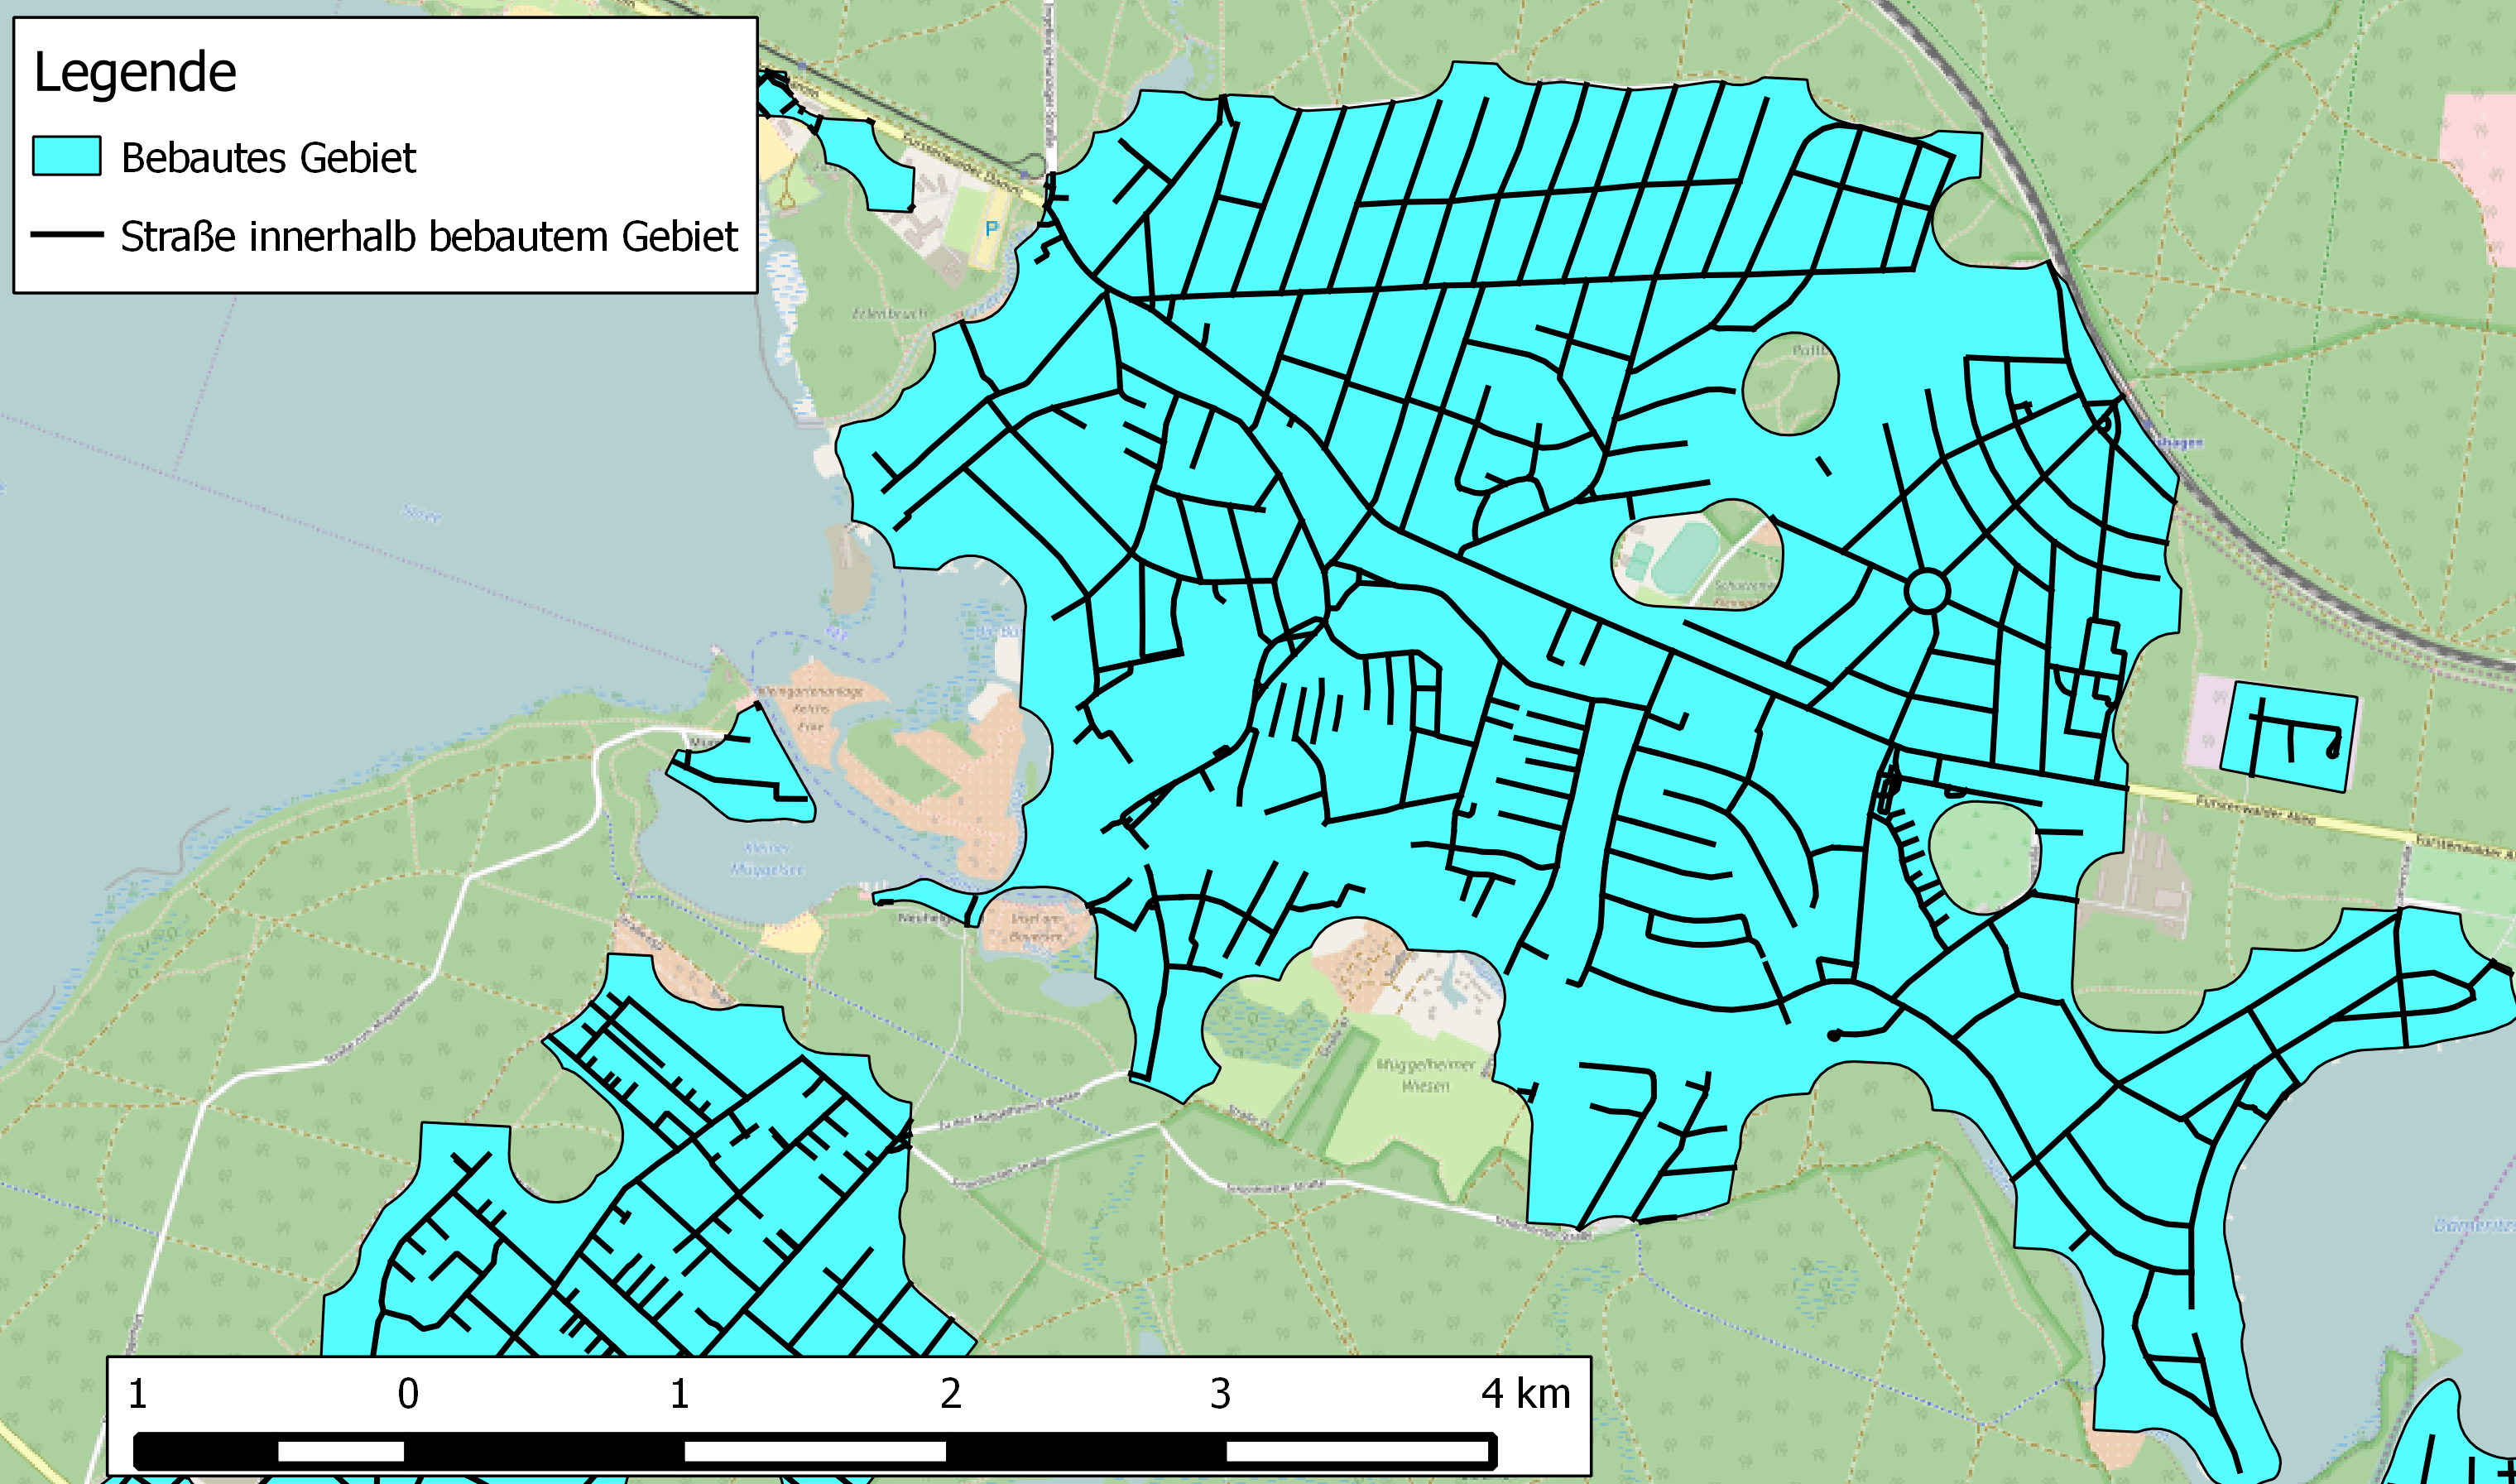
\includegraphics[keepaspectratio,width=0.85\textwidth, height=0.85\textheight]{bilder/Bsp_Lastgebiet}
\caption{Beispiel eines identifizierten Lastgebiets\label{Bsp_Lastgebiet}}
\par\end{centering}
\noindent \begin{centering}
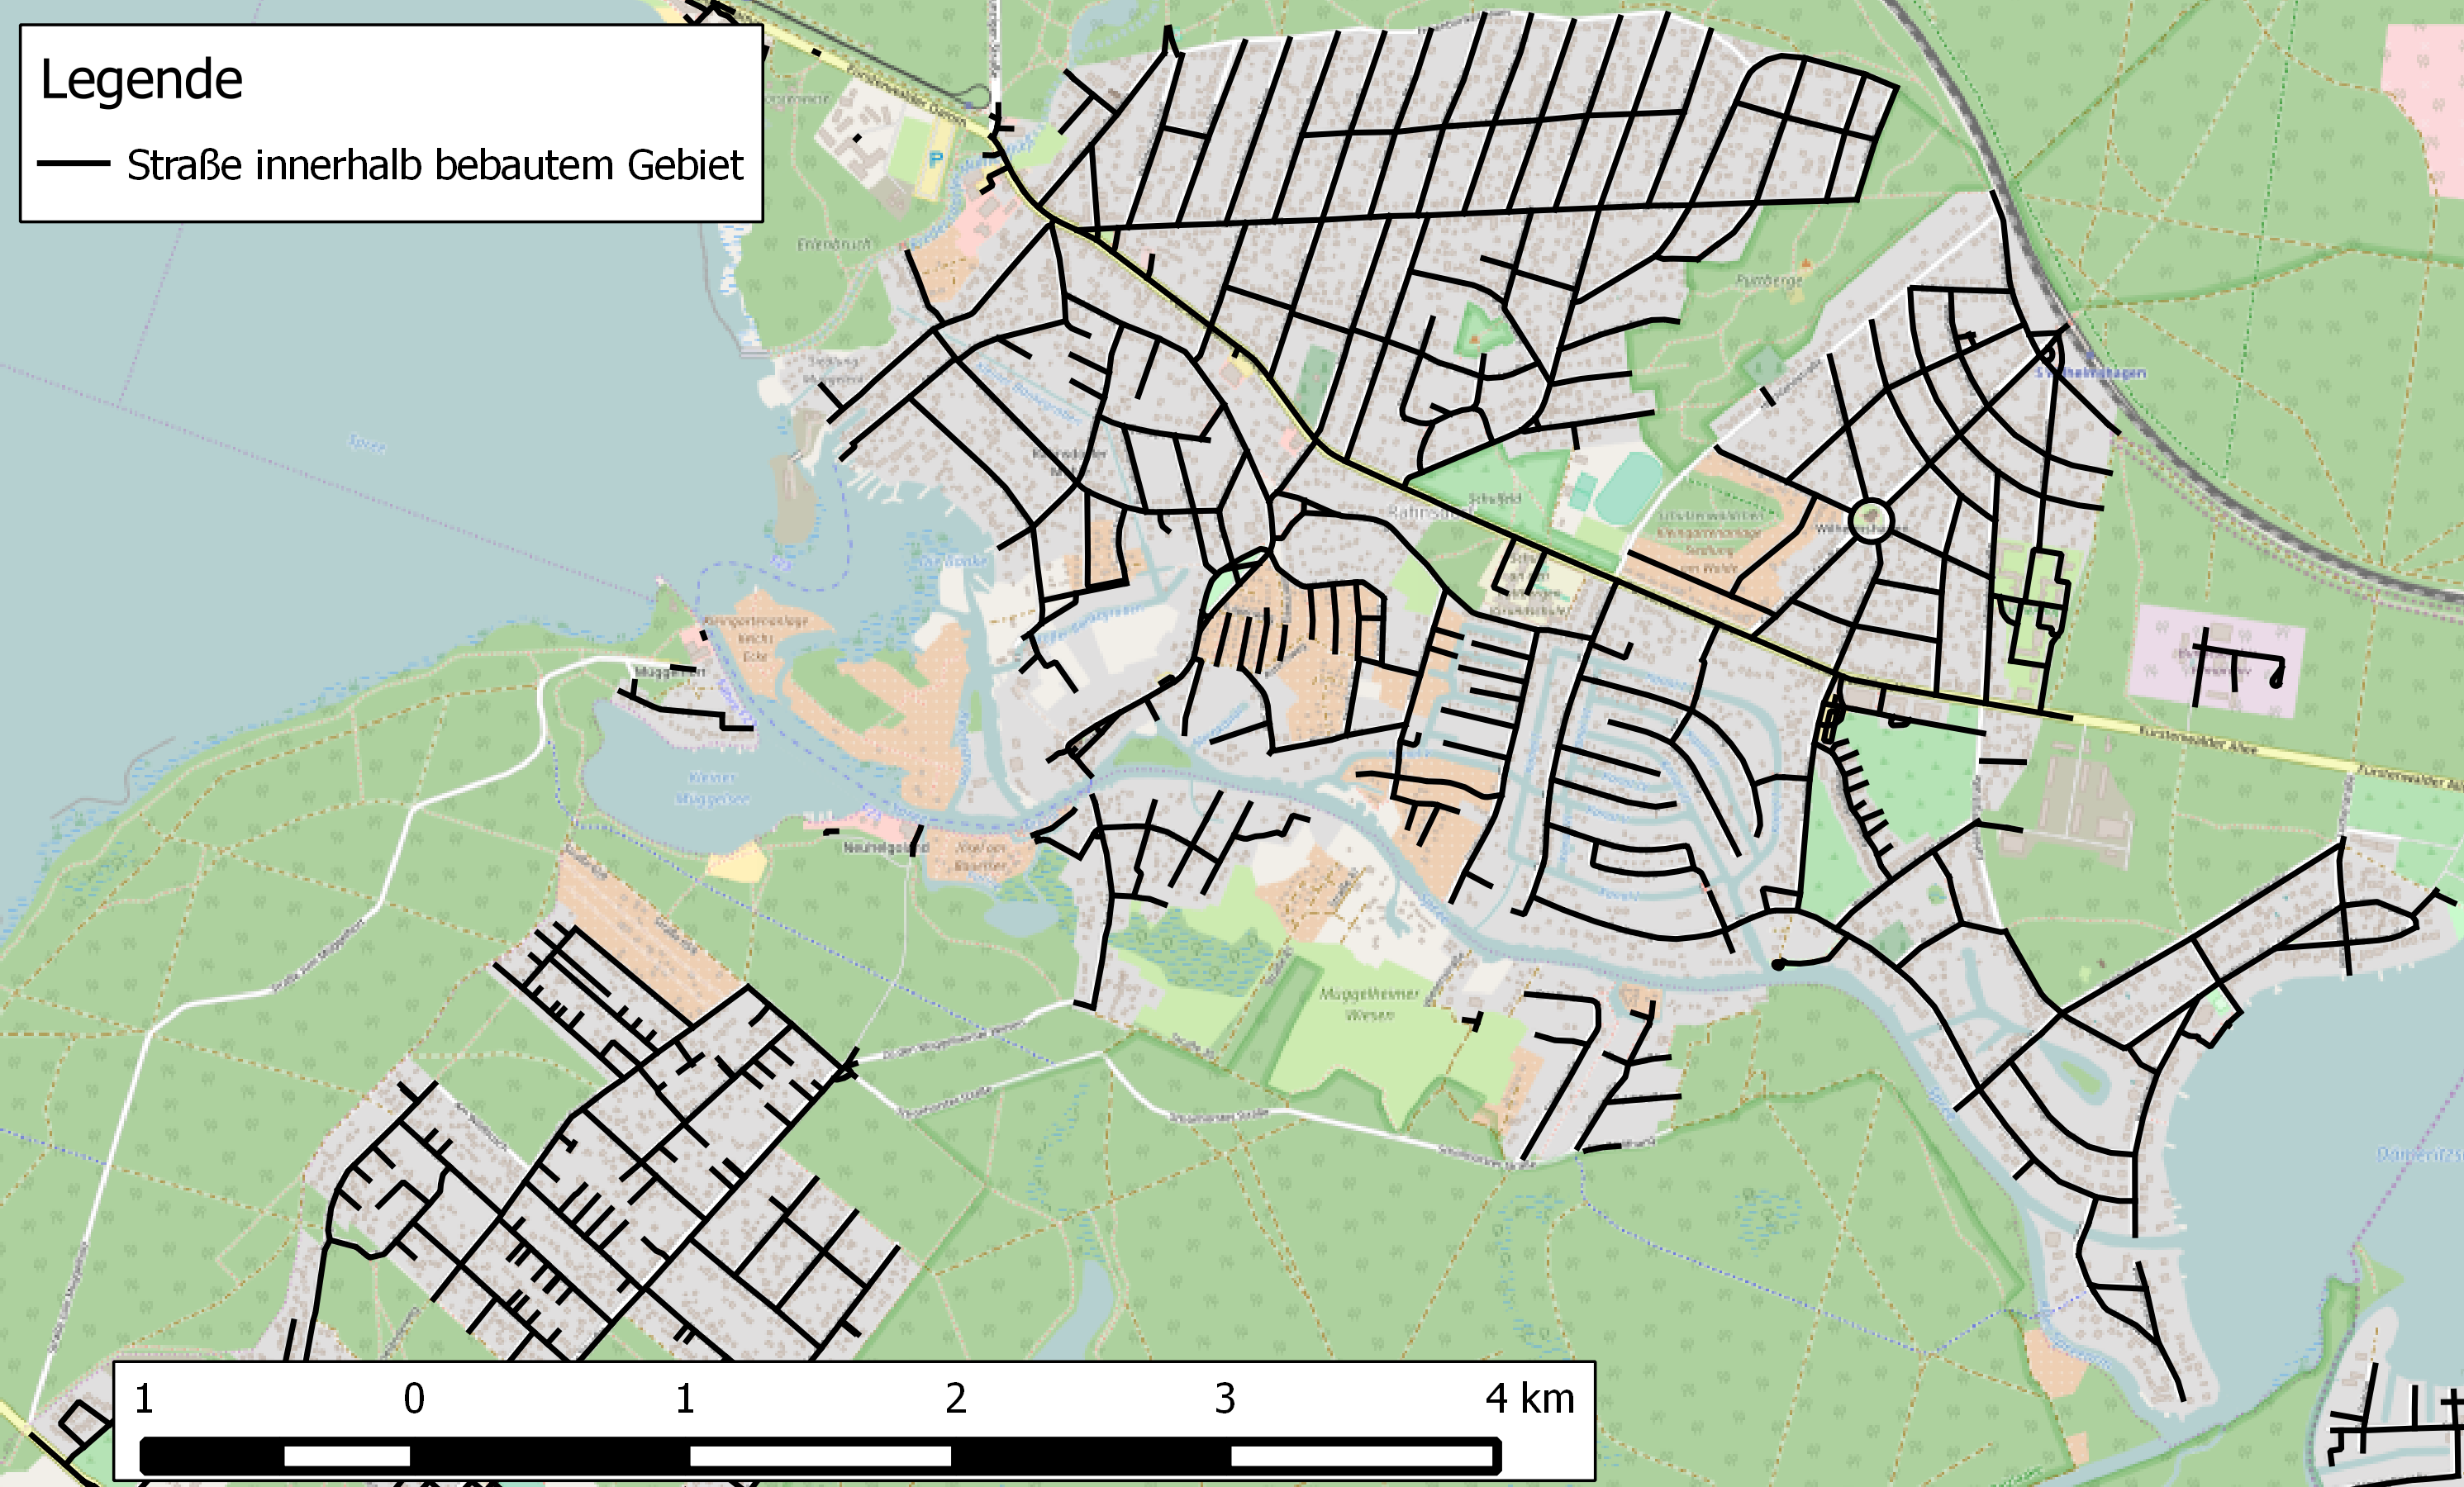
\includegraphics[keepaspectratio,width=0.85\textwidth, height=0.85\textheight]{bilder/Bsp_Lastgebiet_vgl}
\caption{OpenStreetMap-Ansicht des Beispielgebiets\label{Bsp_Lastgebiet_vgl}}
\par\end{centering}

\end{figure} 

\section{Statistische Analyse der Lage von Ortsnetzstationen\label{Statistische Analyse der Lage von Ortsnetzstationen} }

Wie in Kapitel \ref{sec:Aufbau des deutschen Stromnetzes} erklärt, sind neben den Leitungen auch die Ortsnetzstationen ein wichtiger Bestandteil eines Niederspannungsnetzes. Zu diesen sind in OpenStreetMap keine ausreichenden Daten vorhanden. Es wäre jedoch denkbar, dass Zusammenhänge zwischen der Lage von Ortsnetzstationen und in OpenStreetMap vorhandenen Informationen gefunden werden können. Zu diesem Zweck konnten vom Netzbetreiber LVN die Standorte von rund 1100 Ortsnetzstationen im Südwesten Bayerns bezogen werden. Das Netzgebiet von LVN, in dem sich diese Ortsnetzstationen befinden, ist in Abbildung \ref{Netzgebiet_LVN} gezeigt.

\begin{figure}[hb]

\noindent \begin{centering}
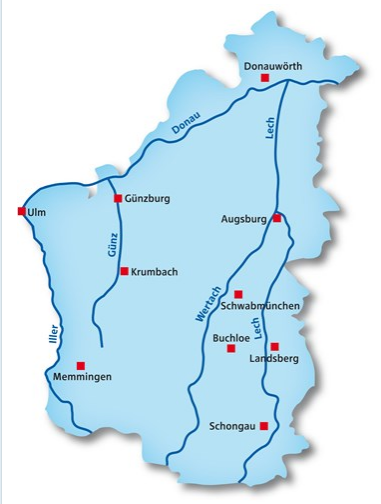
\includegraphics[keepaspectratio,width=\textwidth/2,height=\textheight/2]{bilder/Netzgebiet_LVN}
\caption{Netzgebiet des Netzbetreibers LVN\label{Netzgebiet_LVN}}
\par\end{centering}

\end{figure}

Die in Kapitel \ref{Erstellung eines Netzdatensatzes aus OpenStreetMap-Strassendaten} erzeugten Lastgebiete, in denen sich die 1100 Ortsnetzstationen befinden, werden als Untersuchungsgebiet für die Regressionsanalyse angesehen. In diesen Lastgebieten werden als nächstes 1100 gleichmäßig verteilte Punkte erzeugt, sodass der zu untersuchende Datensatz zu gleichen Teilen aus Ortsnetztransformatoren und aus zufälligen Punkten besteht. für alle 2200 Punkte wird nun eine Reihe von Parametern erhoben, die einfach aus OpenStreetMap-Daten zu ermitteln sind, und für die ein Zusammenhang zur Lage von Ortsnetzstationen denkbar wäre. Diese Parameter sind:

\begin{itemize}
\item Bevölkerung im Umkreis von 50 m
\item Bevölkerung im Umkreis von 100 m
\item Bevölkerung im Umkreis von 250 m
\item Bevölkerung im Umkreis von 500 m
\item Bevölkerung im Umkreis von 1000 m
\item Distanz zur nächsten Straße
\item Distanz zur nächsten Straßenkreuzung
\item Gebäudeanzahl im Umkreis von 50 m
\item Gebäudeanzahl im Umkreis von 100 m
\item Gebäudeanzahl im Umkreis von 250 m
\item Gebäudeanzahl im Umkreis von 500 m
\item Gebäudeanzahl im Umkreis von 1000 m
\item Gesamte Gebäudefläche im Umkreis von 50 m
\item Gesamte Gebäudefläche im Umkreis von 100 m
\item Gesamte Gebäudefläche im Umkreis von 250 m
\item Gesamte Gebäudefläche im Umkreis von 500 m
\item Gesamte Gebäudefläche im Umkreis von 1000 m
\end{itemize}



Aufgrund des Berechnungsverfahrens für einige Parameter können nicht alle Parameter für jeden Punkt berechnet werden. für die Analyse werden im Weiteren nur diejenigen Punkte verwendet, für die jeder Parameter berechnet werden konnte. Anschließend werden die Daten aufgeteilt, in einen Trainings- und einen Testdatensatz, indem die Hälfte aller Punkte zufällig als Trainingsdatensatz ausgewählt wird, und die andere Hälfte den Testdatensatz bildet. Der Testdatensatz wird nicht für die Analyse verwendet, sondern dient dazu, die Ergebnisse später zu validieren. Um einen ersten Überblick über die Verteilungseigenschaften der erhobenen Parameter zu erhalten, werden in einem nächsten Schritt für jeden Parameter Boxplots, Histogramme und Spineplots erstellt, sowie verschiedene Lagemaße bestimmt. Die so erzeugten Diagramme und Maße  sind in Anhang \ref{chap:Plots zur Datenexploration im Vorfeld der logistischen Regression} enthalten. In vielen Fällen ist das Auftreten von deutlichen Ausreißern zu beobachten, die sich um ein Vielfaches vom jeweiligen Mittelwert unterscheiden. Vor allem die Variablen "`Distanz zur nächsten Straße"' und "`Distanz zur nächsten Straßenkreuzung"' sind hiervon betroffen, dort unterscheiden sich einzelne Punkte um mehrere Größenordnungen von den Mittelwerten. Die teilweise sehr hohen Werte der Ausreißer führen dazu, dass die dazugehörigen Histogramme an Aussagekraft verlieren, da der Großteil der Wertebereiche durch nur wenige Balken dargestellt wird. Am wenigsten betroffen davon ist die Gruppe der Variablen, die eine Gebäudeanzahl angeben. Bei diesen beträgt das Maximum meist weniger als das Vierfache des Mittelwertes, und die Histogramme lassen eine linksschiefe Verteilung erkennen.
Die Spineplots zeigen das Verhalten der Variablen im Bezug auf die abhängige Variable (Vorhandensein einer Ortsnetzstation). Sämtliche Variablen, die eine Bevölkerung angeben, weisen sehr gleichmäßige Spineplots auf, bei denen kein Zusammenhang zur abhängigen Variable sichtbar ist. Bei der Variable "`Distanz zur nächsten Straße"' lässt sich dagegen ein leichter negativer Zusammenhang erkennen. Auch bei der Variable "`Distanz zur nächsten Straßenkreuzung"' lässt sich dieser Zusammenhang vermuten, allerdings nur sehr undeutlich. Ein klar erkennbarer positiver Zusammenhang ist dagegen bei der Variable zu beobachten, die die Gebäudeanzahl in einem Radius von 50 m beschreibt. Sämtliche anderen Variablen, die eine Gebäudeanzahl beschreiben, lassen diesen Zusammenhang ebenfalls vermuten, allerdings in deutlich schwächerer Form. Ebenfalls ist ein positiver Zusammenhang bei allen Variablen der Gebäudefläche vorhanden, der bei hohen Radien schwächer wird. Die folgenden Variablen erscheinen aufgrund der Betrachtung der Spineplots am vielversprechendsten für das Finden eines Zusammenhangs mit der abhängigen Variable:

\begin{itemize}
\item Distanz zur nächsten Straße
\item Gebäudeanzahl im Umkreis von 50 m
\item Gesamte Gebäudefläche im Umkreis von 100 m
\end{itemize}

Die dazugehörigen Spineplots sind in den Abbildungen \ref{Spine6}, \ref{Spine8} und \ref{Spine14} dargestellt.

\begin{figure}[p]

\noindent \begin{centering}
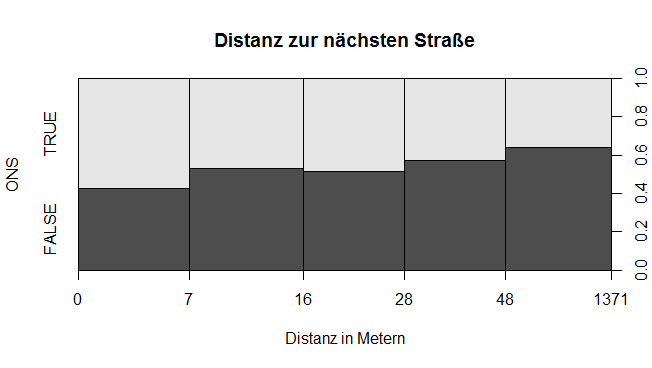
\includegraphics[keepaspectratio,width=0.7\textwidth,height=0.7\textheight/2]{bilder/Anhang_A/Spine6}
\caption{Spineplot des Parameters "`Distanz zur nächsten Straße"'\label{Spine6}}
\par\end{centering}

\end{figure}

\begin{figure}

\noindent \begin{centering}
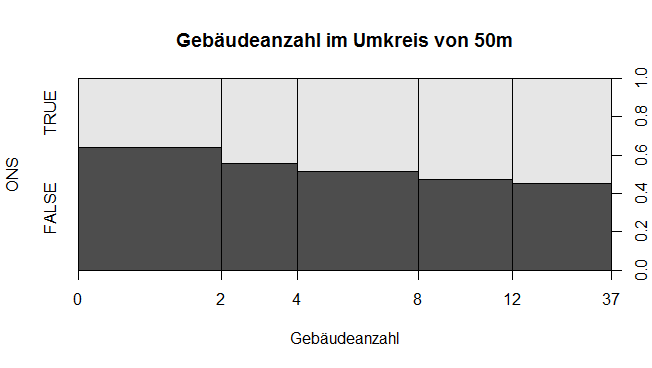
\includegraphics[keepaspectratio,width=0.7\textwidth,height=0.7\textheight]{bilder/Anhang_A/Spine8}
\caption{Spineplot des Parameters "`Gebäudeanzahl im Umkreis von 50m"'\label{Spine8}}
\par\end{centering}

\end{figure}

\begin{figure}

\noindent \begin{centering}
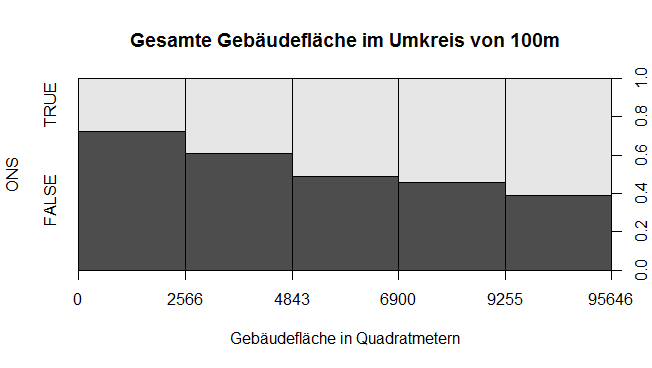
\includegraphics[keepaspectratio,width=0.7\textwidth,height=0.7\textheight]{bilder/Anhang_A/Spine14}
\caption{Spineplot des Parameters "`Gesamte Gebäudefläche im Umkreis von 100m"'\label{Spine14}}
\par\end{centering}

\end{figure}

Da es die große Anzahl an möglichen Prediktoren jedoch sehr schwer macht, visuell die optimalen Parameter auszuwählen, wird dafür eine automatisierte Stepwise Variable Selection per AIC durchgeführt. Der AIC (Akaike Information Criterion) ist ein Maß zum Vergleich der Güte verschiedener Modelle. Je kleiner der AIC, desto besser passt das Modell zu den Daten. Der AIC bestraft außerdem die Größe eines Modells, was bedeutet, dass Modelle mit weniger Parametern bessere AIC-Werte erhalten als gleichwertige Modelle mit mehr Parametern. Bei der Stepwise Variable Selection wird vom Nullmodell ausgegangen, welches besagt, dass kein Parameter mit der abhängigen Variable korreliert ist. Zu diesem Modell wird schrittweise jeweils derjenige Parameter hinzugefügt, der die stärkste Verringerung des AIC zur Folge hat, und dies solange wiederholt, bis kein zusätzlicher Parameter mehr den AIC senken würde. Diese Technik wird auf ein GLM (Generalized Linear Model) angewandt, welches durch folgende Formel ausgedrückt wird:

\begin{equation}
P(event) = \frac{1}{1-e^{(-z)}}
\label{formel2} 
\end{equation}
\citep{Fielding2007}

Dabei steht z für eine Reihe von Prediktoren $x_n$ und deren Gewichtungen $b_n$ in der Form:

\begin{equation}
z = b_0+b_1x_1+b_2x_2+b_3x_3+...+b_nx_n
\label{formel3} 
\end{equation}
\citep{Fielding2007}

und P(event) für die Wahrscheinlichkeit, dass an dem betrachteten Punkt eine ONS vorhanden ist.
Die Beziehung zwischen P(event) und den Prediktoren ist dabei zunächst nicht linear. Es wird eine lineare Beziehung hergestellt, indem P(event) in logits umgewandelt wird: 

\begin{equation}
logit[P(event)] = log[\frac{P(event)}{P(no event)}]
\label{formel4} 
\end{equation}
\citep{Fielding2007}


Für die mittels der Stepwise Variable Selection ermittelten Prediktoren wird anschließend der Varianzinflationsfaktor (VIF) gebildet. Er gibt an, um welchen Faktor die Varianz durch lineare Abhängigkeit vergrößert wird. Möglichst kleine Werte sind für den VIF also wünschenswert. Werte des VIF von unter 10 gelten als unproblematisch. Alle Prediktoren, deren VIF oberhalb 10 liegt, werden daher aus dem Modell entfernt.


\section{Modellierung der Ortsnetzstationen\label{Modellierung der Ortsnetzstationen}}

\subsection{Bestimmung der Anzahl an Ortsnetzstationen }


Auf Grundlage der Ergebnisse der logistischen Regression werden möglichst günstige Standorte für Ortsnetzstationen innerhalb der in Kapitel \ref{Erstellung eines Netzdatensatzes aus OpenStreetMap-Strassendaten} erzeugten Lastgebiete gesucht. Dafür muss zunächst die Anzahl an Ortsnetzstationen pro Lastgebiet abgeschätzt werden. Zu diesem Zweck wird die Größe eines durchschnittlichen Einzugsgebiets einer Ortsnetzstation anhand von Angaben zur durchschnittlichen Stranglänge in einem Niederspannungsnetz abgeschätzt.
\citet{Mohrmann2012} geben für verschiedene Siedlungstypen charakteristische Stranglängen an.Da ein großer Teil der betrachteten Ortschaften dörfliche Strukturen aufweist und Dörfer im Gegensatz zu Städten aufgrund ihrer Änderungen im Einspeiseverhalten auch am wichtigsten für die Analyse deutscher Niederspannungsnetze sind, wurde die Angabe für den Typ "`Siedlungen niedriger Dichte"' für die vorliegende Arbeit übernommen. Demnach weist ein typischer Niederspannungsstrang in einem solchen Gebiet eine Länge von 200-300 m auf. Aus dieser Angabe wurde die Größe eines durchschnittlichen Einzugsgebietes abgeleitet. Bei Annahme eines Radialnetzes, wie es nach Heuck in den meisten Fällen in der Niederspannung vorkommt, kann man von einer annähernd kreisförmigen Form des Einzugsgebiets ausgehen, sodass also dessen Fläche $\pi*r^2$ beträgt, wobei r den Radius des Gebietes angibt \citep{Heuck2013}. Der Radius entspräche der typischen Stranglänge von 200-300 m, wenn man davon ausginge, dass ein Strang gerade von der Ortsnetzstation nach außen verlaufen würde. Da Leitungsstränge aber im Normalfall nicht exakt gerade verlaufen, wird der tatsächliche Radius geringer sein als die durchschnittliche Stranglänge. Nach einer Stichprobenuntersuchung sämtlicher Niederspannungsstränge in einem Dorf im Netzgebiet des LVN beträgt die Länge von Leitungssträngen dort 72\% im Vergleich zur Luftlinienentfernung zwischen Start- und Endpunkt des Strangs. Der Radius eines Einzugsgebiets einer Ortsnetzstation sollte daher um diesen Anteil geringer ausfallen als die typische Stranglänge und ergibt sich somit zu durchschnittlich 180 m. Daraus lässt sich eine Fläche von ca. 10 Hektar ableiten. 
Um nun die wahrscheinlichste Anzahl an Ortsnetzstationen innerhalb eines Lastgebietes zu ermitteln, wird dieses mit fiktiven Einzugsgebieten von 10 ha Größe gefällt, wie in Abbildung \ref{ONS_Anzahl_1} beispielhaft dargestellt. Aus Gründen einer einfacheren Durchführung werden dabei quadratische anstatt kreisförmige Gebiete verwendet. Alle Mittelpunkte der fiktiven Einzugsgebiete, die innerhalb des Lastgebietes liegen, werden sodann als Ortsnetzstationen gezählt (siehe Abbildung \ref{ONS_Anzahl_2}). Je nach Form des Lastgebietes kann es dabei leicht dazu kommen, dass zu wenige Ortsnetzstationen gezählt werden. Um dem entgegenzuwirken, wird geprüft, ob es innerhalb des Lastgebietes Bereiche gibt, die außergewöhnlich weit weg von der nächsten fiktiven Ortsnetzstation liegen. Dafür wird abermals ein Wert von \citet{Mohrmann2012} genutzt: Die von ihnen gefundene größte Stranglänge in Siedlungen niedriger Dichte beträgt 1500 m, es ist also anzunehmen, dass kein Punkt innerhalb eines Lastgebietes weiter als 1500 m entfernt von der nächsten Ortsnetzstation liegen kann. Auch dies gilt nur wieder im unwahrscheinlichen Fall eines exakt gerade verlaufenden Stranges, sodass $0,72*1500 m = 1080 m$ vermutlich eine bessere Näherung ergibt. Alle Gebiete, die weiter als 1080 m von der nächsten Ortsnetzstation entfernt sind, werden also, wie in Abbildung \ref{ONS_Anzahl_3} gezeigt, ausgewählt und in deren Mittelpunkt eine weitere fiktive Ortsnetzstation gesetzt. Als letztes werden nun sämtliche der fiktiven Ortsnetzstationen in einem Lastgebiet gezählt, um geschätzte Anzahl an Ortsnetzstationen in diesem Gebiet zu erhalten.

\begin{figure} 

\noindent \begin{centering}
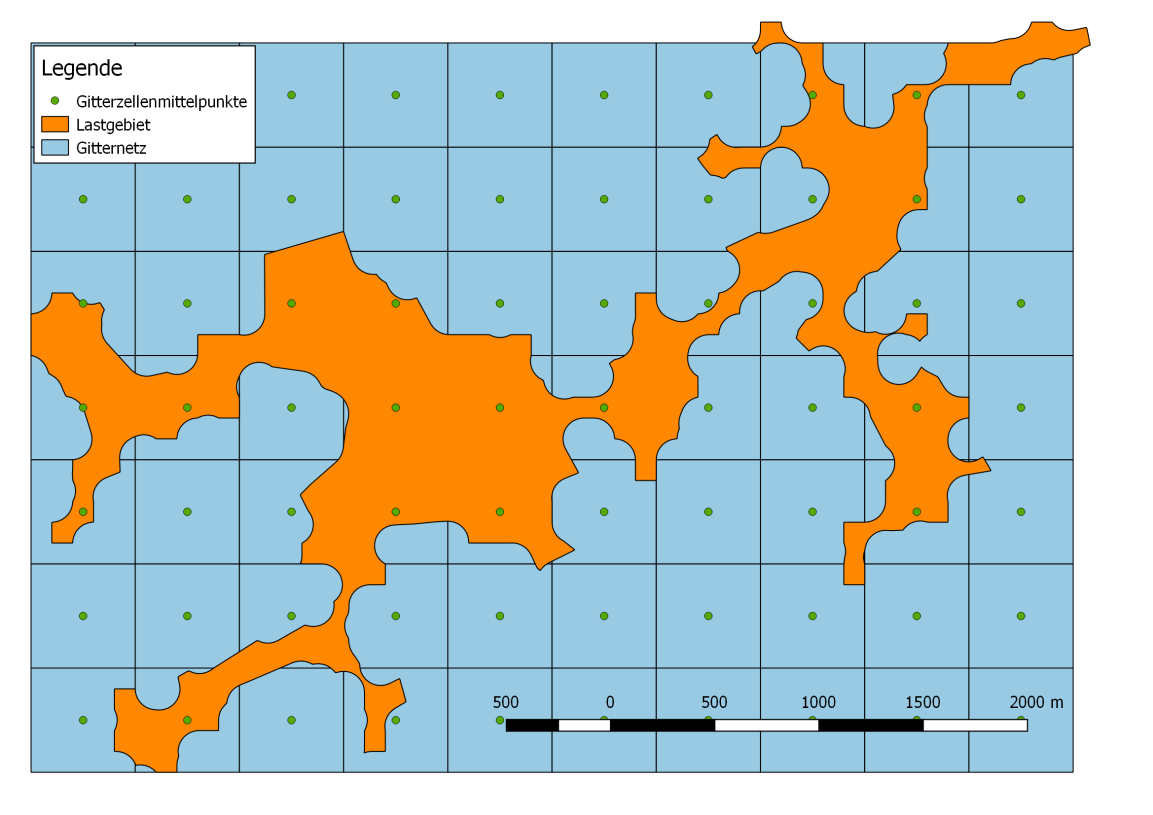
\includegraphics[keepaspectratio,width=\textwidth,height=\textheight]{bilder/ONS_Anzahl_1}
\caption{Füllung eines Lastgebiets mit fiktiven Einzugsgebieten - Schritt 1\label{ONS_Anzahl_1}}
\par\end{centering}

\end{figure}

\begin{figure} [p]

\noindent \begin{centering}
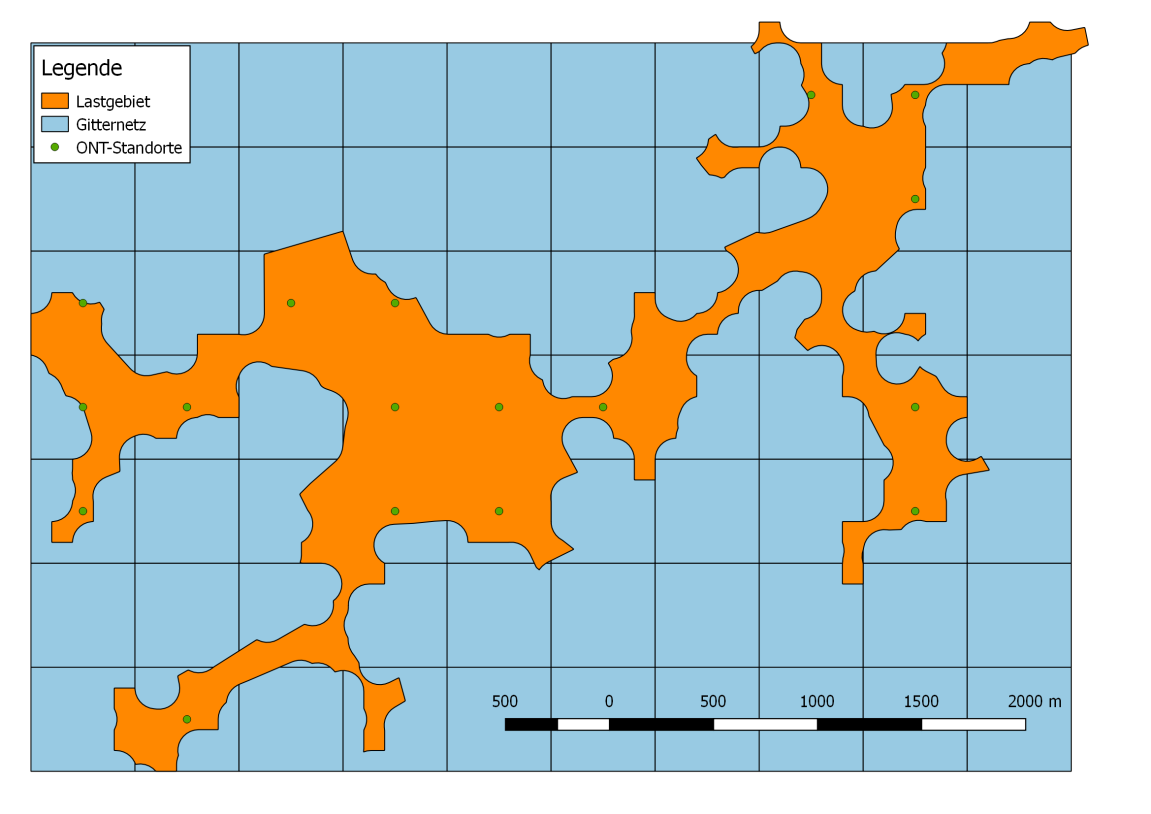
\includegraphics[keepaspectratio,width=\textwidth,height=\textheight]{bilder/ONS_Anzahl_2}
\caption{Füllung eines Lastgebiets mit fiktiven Einzugsgebieten - Schritt 2\label{ONS_Anzahl_2}}
\par\end{centering}

\end{figure}


\begin{figure}

\noindent \begin{centering}
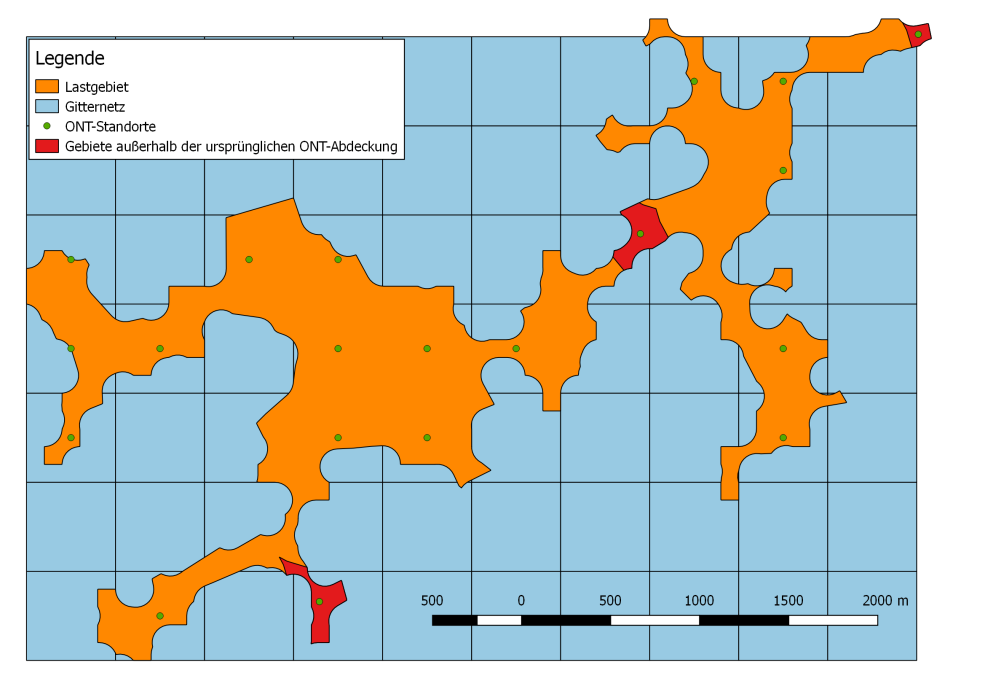
\includegraphics[keepaspectratio,width=\textwidth,height=\textheight]{bilder/ONS_Anzahl_3}
\caption{Füllung eines Lastgebiets mit fiktiven Einzugsgebieten - Schritt 3\label{ONS_Anzahl_3}}
\par\end{centering}

\end{figure}

\subsection{Positionierung der Ortsnetzstationen }

Die finale Positionierung der Ortsnetzstationen erfolgt auf dem Straßennetz. Es wird versucht, die im vorigen Kapitel geschätzte Anzahl an Ortsnetzstationen möglichst der Realität entsprechend über das betreffende Gebiet zu verteilen. Dabei wird zunächst eine gleichmäßige Verteilung der Ortsnetzstationen angestrebt, da lange Wege zwischen Transformator und Verbraucher elektrotechnisch ungünstig sind und verstärkte Leitungen benötigen, was sich negativ auf die Wirtschaftlichkeit auswirkt. Das Problem, die Ortsnetzstationen gleichmäßig auf dem Straßennetz zu positionieren, ist dem in der Graphentheorie bekannten metrischen k-center-Problem sehr ähnlich. Bei diesem geht es darum, auf einem Graphen eine vorgegebene Anzahl von Zentren auszuwählen, sodass der maximale Abstand eines Knotens zu seinem nächsten Zentrum möglichst klein ist. Das k-center-Problem ist NP-schwer, das heißt es gibt wahrscheinlich keinen schnellen Algorithmus, der eine optimale Lösung findet. Schnell bedeutet hier, dass die Laufzeit polynomiell ist, also mit der Größe der Eingabe nur vergleichsweise langsam ansteigt \citep{Wanka2006}. Algorithmen, deren Laufzeit nicht polynomiell ist, sind meist zu langsam, um für praktische Probleme von Nutzen zu sein. Eine Annäherung an die optimale Lösung des k-center-Problems mit polynomieller Laufzeit ist durch folgenden Algorithmus angegeben: 

\begin{algorithm} [ht]

Wähle einen beliebigen Knoten als erstes Zentrum aus\;
\While{gewünschte Anzahl an Zentren noch nicht erreicht}{
Wähle das nächste Zentrum so, dass seine Distanz zu den bereits bestehenden Knoten maximal ist.
}
\caption{Schnelle Lösung des k-center-Problems\label{Schnelle Losung des k-center-Problems}}
\end{algorithm}

Für die mit obigem Algorithmus ausgewählten Zentren beträgt der maximale Abstand zwischen einem Knoten und seinem nächsten Zentrum höchstens das Zweifache des Abstandes, der sich bei der optimalen Lösung ergibt. Ein genauerer schneller Algorithmus als der oben vorgestellte ist nicht bekannt \citep{Williamson2010}, daher wurde er für den vorliegenden Zweck als Grundlage verwendet. Für die Positionierung der Ortsnetzstationen liegen jedoch zusätzliche Informationen vor, die möglicherweise für eine Verbesserung der Genauigkeit im Hinblick auf die reale Verteilung der Ortsnetzstationen verwendet werden können. Diese Informationen sind die in Kapitel \ref{Statistische Analyse der Lage von Ortsnetzstationen} erhobenen Prediktoren. Anstatt eine näherungsweise gleichmäßige Verteilung anzustreben, wird der obige Algorithmus so abgewandelt, dass die Auswahl der Zentren sich an den Werten der Prediktoren orientiert. Dies geschieht auf folgende Weise: Um den Positionierungsalgorithmus ausführen zu können, wird das Straßennetz zuerst mit Hilfe der Python-Programmiersprache in einen Graphen umgewandelt. Jede Kante des Straßennetzes bildet eine Kante, deren Start-und Endpunkte bilden die Knoten des Graphen (siehe Abbildung \ref{ONS_Positionierung_2}). Jeder Knoten ist ein möglicher Standort einer Ortsnetzstation und ist initial als undominiert markiert. Für jeden Knoten werden außerdem die Werte der in Kapitel \ref{Erstellung eines Netzdatensatzes aus OpenStreetMap-Strassendaten} bestimmten Modellparameter ermittelt und daraus der Exponent z aus Formel \ref{formel2} bestimmt. Dieser kann als Maß für die Wahrscheinlichkeit, dass es sich bei dem Knoten um eine Ortsnetzstation handelt, betrachtet werden. Der erste Schritt des Algorithmus besteht nun darin, denjenigen Knoten auszuwählen, der den höchsten Wert für z aufweist, und diesen als Ortsnetzstation zu markieren (Abbildung \ref{ONS_Positionierung_3}). Als Nächstes werden sämtliche Knoten, die von der neu ausgewählten Ortsnetzstation aus unter Annahme eines durchschnittlich großen Ortsnetzes versorgt werden können, als dominiert markiert und dieser Ortsnetzstation zugewiesen (Abbildung \ref{ONS_Positionierung_4}). Diese Zuweisung erfolgt auf Grundlage der zuvor geschätzten durchschnittlichen Länge eines Niederspannungsstrangs. Auf den verbleibenden, als undominiert markierten Knoten, wird nun der Algorithmus erneut ausgeführt, es wird also wiederum der Knoten mit dem höchsten Wert für z ausgewählt, als Ortsnetzstation gekennzeichnet, und die Knoten in dessen Einzugsgebiet als dominiert markiert (Abbildung  \ref{ONS_Positionierung_5}). Dies wird solange wiederholt, bis die gewünschte Anzahl an Ortsnetzstationen positioniert worden ist. Zu Zwecken der Übersichtlichkeit ist der beschriebene Vorgang hier nochmals in Pseudocode-Schreibweise dargestellt:

\begin{algorithm} [H]
Wähle den Knoten als erstes Zentrum aus, der die höchste Wahrscheinlichkeit aufweist\;
\While{gewünschte Anzahl an Zentren noch nicht erreicht}{
Entferne alle Knoten, die sich im Einzugsbereich der bestehenden Zentren befinden, aus der Auswahl\;
Wähle den Knoten als nächstes Zentrum, der die höchste Wahrscheinlichkeit aufweist
}
\caption{Positionierung der Ortsnetzstationen\label{Positionierung der Ortsnetzstationen}}
\end{algorithm}

\begin{figure} [h]

\noindent \begin{centering} 
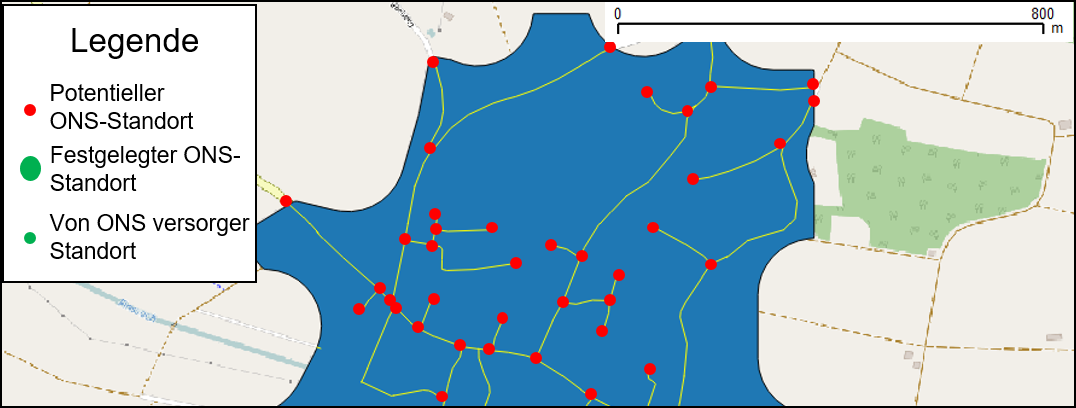
\includegraphics[keepaspectratio,width=\textwidth,height=\textheight]{bilder/ONS_Positionierung_2}
\caption{Positionierung von Ortsnetzstationen - Schritt 1\label{ONS_Positionierung_2}}
\par\end{centering}

\end{figure}

\begin{figure} 

\noindent \begin{centering}
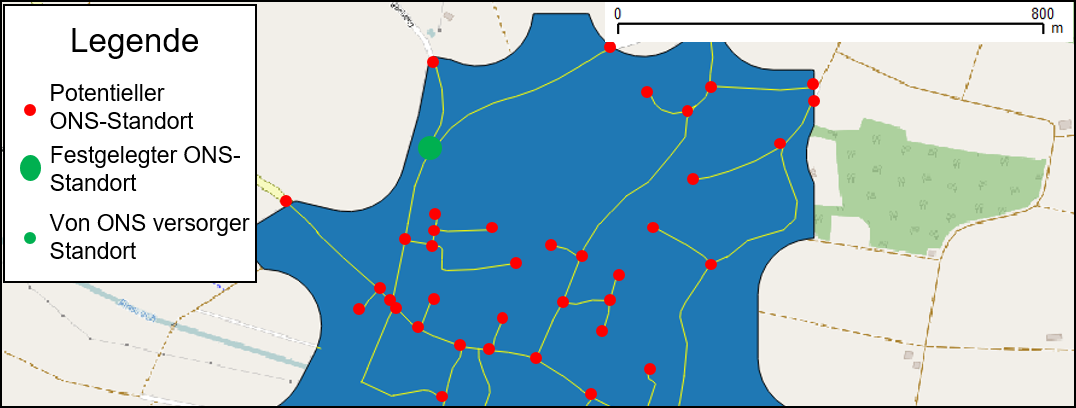
\includegraphics[keepaspectratio,width=\textwidth,height=\textheight]{bilder/ONS_Positionierung_3}
\caption{Positionierung von Ortsnetzstationen - Schritt 2\label{ONS_Positionierung_3}}
\par\end{centering}

\end{figure}

\begin{figure} 

\noindent \begin{centering}
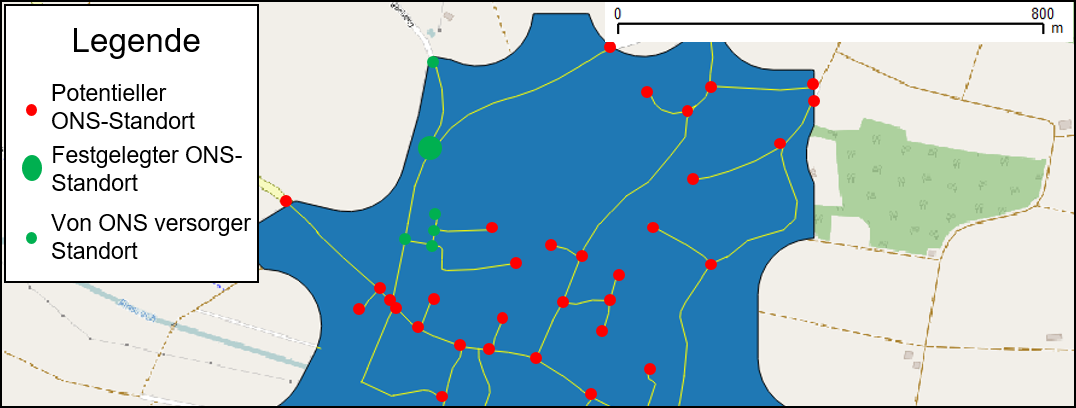
\includegraphics[keepaspectratio,width=\textwidth,height=\textheight]{bilder/ONS_Positionierung_4}
\caption{Positionierung von Ortsnetzstationen - Schritt 3\label{ONS_Positionierung_4}}
\par\end{centering}

\end{figure}

\begin{figure} 

\noindent \begin{centering}
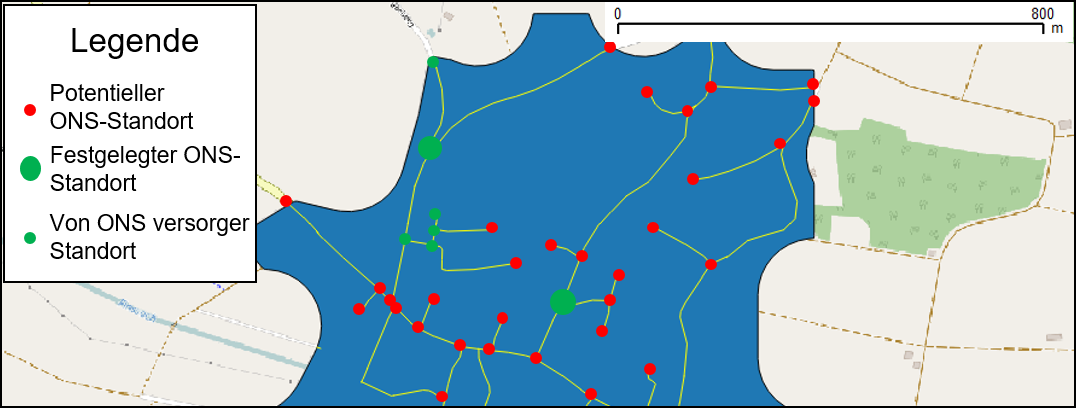
\includegraphics[keepaspectratio,width=\textwidth,height=\textheight]{bilder/ONS_Positionierung_5}
\caption{Positionierung von Ortsnetzstationen - Schritt 4\label{ONS_Positionierung_5}}
\par\end{centering}

\end{figure}

\newpage

\section{Validierung\label{Validierung}}

Alle deutschen Netzbetreiber sind dazu verpflichtet, Strukturdaten zu ihren Netzen zu veröffentlichen. Zu diesen Strukturdaten zählt unter anderem die gesamte Leitungslänge im Netzgebiet. Diese Angabe wurde zur Validierung der aus den OpenStreetMap-Daten erzeugten Netze verwendet. Dazu wurden von 20 Verteilnetzbetreibern die gesamte Länge der Kabelleitungen in deren Netzgebiet recherchiert. Nur drei dieser Betreiber stellten Daten zur Kabellänge ohne Hausanschlüsse zur Verfügung, daher wurden in den Netzgebieten dieser drei Betreiber die gesamte Länge der modellierten Netze erhoben und die Längen miteinander verglichen. Die drei Netzbetreiber sind:

\begin{itemize}
\item EWR Netze
\item Enervie Vernetzt
\item Energie Waldeck Frankenberg
\end{itemize}

Über die Webseiten dieser Netzbetreiber wurden Karten von deren Netzgebieten im pdf-Format bezogen. Diese Karten wurden georeferenziert und damit die Straßen identifiziert, die in diesen Netzgebieten liegen. Die gesamte Länge dieser Straßen wurde pro Netzgebiet bestimmt. Im Kapitel \ref{chap:Ergebnisse} werden die Leitungslängen miteinander verglichen.

Mittels des in Kapitel \ref{Statistische Analyse der Lage von Ortsnetzstationen} vorgestellten Verfahrens wurden Transformator-Standorte für alle Lastgebiete des Untersuchungsgebiets generiert, und die Anzahl der modellierten und der realen Ortsnetzstationen für jedes Lastgebiet miteinander verglichen. Außerdem wurde für alle Ortsnetzstationen im Testdatensatz deren Position mit der Position der am nächsten liegenden modellierten Ortsnetzstation verglichen. Im Kapitel \ref{chap:Ergebnisse} werden die Ergebnisse der Validierung vorgestellt.

\chapter{Ergebnisse\label{chap:Ergebnisse} }

\section{Ortsnetzstationen}
Sämtliche untersuchten Parameter mit Ausnahme des Parameters "`Gebäudefläche im Umkreis von 50 m"' würden als Ergebnis der Stepwise Variable Selection zu einer Verbesserung des Modells führen. Es zeigt sich, dass einige der gewählten Prediktoren VIF-Werte deutlich über 10 aufweisen. Diese sind:

\begin{itemize}
\item Bevölkerung im Umkreis von 250 m
\item Bevölkerung im Umkreis von 500 m
\item Bevölkerung im Umkreis von 1000 m
\item Gebäudeanzahl im Umkreis von 100 m
\item Gebäudeanzahl im Umkreis von 250 m
\item Gebäudeanzahl im Umkreis von 500 m
\item Gebäudeanzahl im Umkreis von 1000 m
\item Gesamte Gebäudefläche im Umkreis von 500 m
\item Gesamte Gebäudefläche im Umkreis von 1000 m
\end{itemize}

Die oben aufgelisteten Prediktoren führen zu starker Kollinearität im Modell und werden deshalb aus dem Modell entfernt. Die übrigen, finalen Prediktoren und ihre Koeffizienten sind im Folgenden dargestellt:

\begin{itemize}
\item Bevölkerung im Umkreis von 50 m : $5.662*10^{-03}$
\item Bevölkerung im Umkreis von 100 m: $-1.099*10^{-03}$
\item Distanz zur nächsten Straße: $-3.498*10^{-03}$
\item Distanz zur nächsten Straßenkreuzung: $-3.530*10^{-03}$
\item Gebäudeanzahl im Umkreis von 50 m: $3.480*10^{-03}$
\item Gesamte Gebäudefläche im Umkreis von 100 m: $3.240*10^{-05}$
\item Gesamte Gebäudefläche im Umkreis von 250 m: $8.963*10^{-06}$
\end{itemize}

\section{Validierung der Leitungen}

In Tabelle \ref{Tab_Leitungsvalidierung} ist eine Übersicht der zur Validierung verwendeten Netzgebiete dargestellt. In jedem der drei betrachteten Netzgebiete ist die Länge der Niederspannungs-Stromleitungen deutlich höher als die Länge der zur Abbildung der Leitungen verwendeten Straßen aus OpenStreetMap. Zwischen den beiden Längen ergibt sich ein durchschnittlicher Fehlbetrag von 1096 Kilometern innerhalb eines Netzgebiets, bezogen auf die Fläche ergibt sich ein durchschnittlicher Fehlbetrag von 1,05 Kilometern pro Quadratkilometer.
Die betrachtete Straßenlänge beträgt durchschnittlich 67\% der tatsächlichen Leitungslänge.

\begin{table}

\noindent \begin{centering}
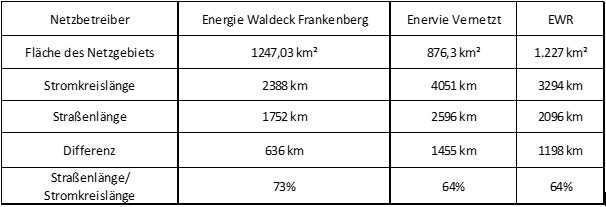
\includegraphics[keepaspectratio,width=\textwidth,height=\textheight]{bilder/Tabelle_Leitungsvalidierung}
\caption{Vergleich der tatsächlichen mit den modellierten Leitungslängen in verschiedenen Netzgebieten\label{Tab_Leitungsvalidierung}}
\par\end{centering}

\end{table}

\section{Validierung der Ortsnetzstationen}

\subsection{Anzahl der Ortsnetzstationen}

Im gesamten Untersuchungsgebiet stehen insgesamt 1080 Ortsnetzstationen. Im selben Gebiet wurden mit den beschriebenen Methoden 953 künstliche Ortsnetzstationen erzeugt, was einen Unterschied zwischen Realität und Modell von 127 Ortsnetzstationen, oder 11,76\%,  ergibt. In Abbildung \ref{plot_realmodons} sind für jedes betrachtete Lastgebiet die Anzahl der modellierten gegen die Anzahl der realen Ortsnetzstationen aufgetragen. Für die Abweichungen der beiden Anzahlen voneinander zeigen die Abbildungen \ref{hist_diff} und \ref{hist_diff_abs} das Histogramm der Verteilung, wobei in Abbildung \ref{hist_diff} die Differenz zwischen realer und modellierter Anzahl und in Abbildung \ref{hist_diff_abs} der Betrag dieser Differenz dargestellt ist.

\begin{figure} 

\noindent \begin{centering}
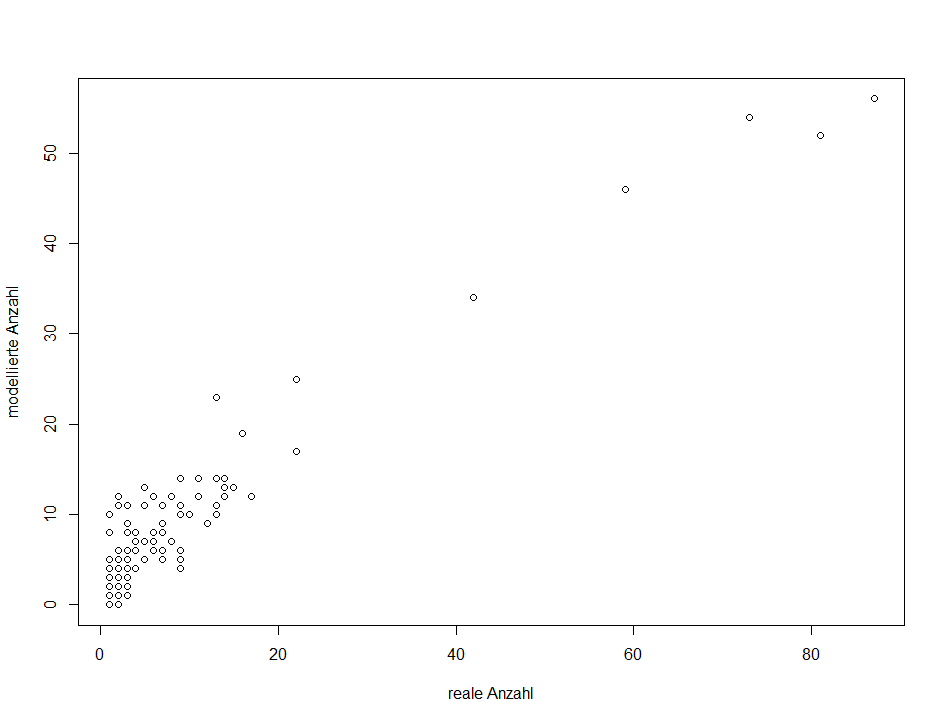
\includegraphics[keepaspectratio,width=0.8\textwidth,height=0.8\textheight]{bilder/plot_realmodons}
\caption{Reale und modellierte Anzahlen der Ortsnetzstationen auf Ebene der Lastgebiete\label{plot_realmodons}}
\par\end{centering}

\end{figure}

\begin{figure}

\noindent \begin{centering}
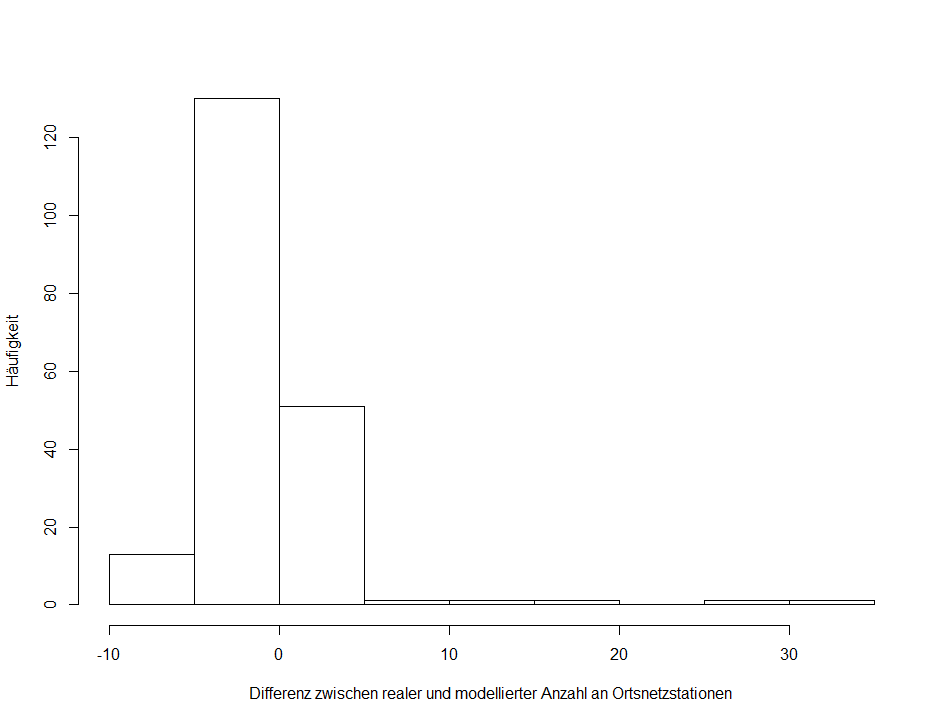
\includegraphics[keepaspectratio,width=0.8\textwidth,height=0.8\textheight]{bilder/hist_diff}
\caption{Histogramm der Unterschiede zwischen realer und modellierter Anzahl an Ortsnetzstationen\label{hist_diff}}
\par\end{centering}

\end{figure}

\begin{figure}

\noindent \begin{centering}
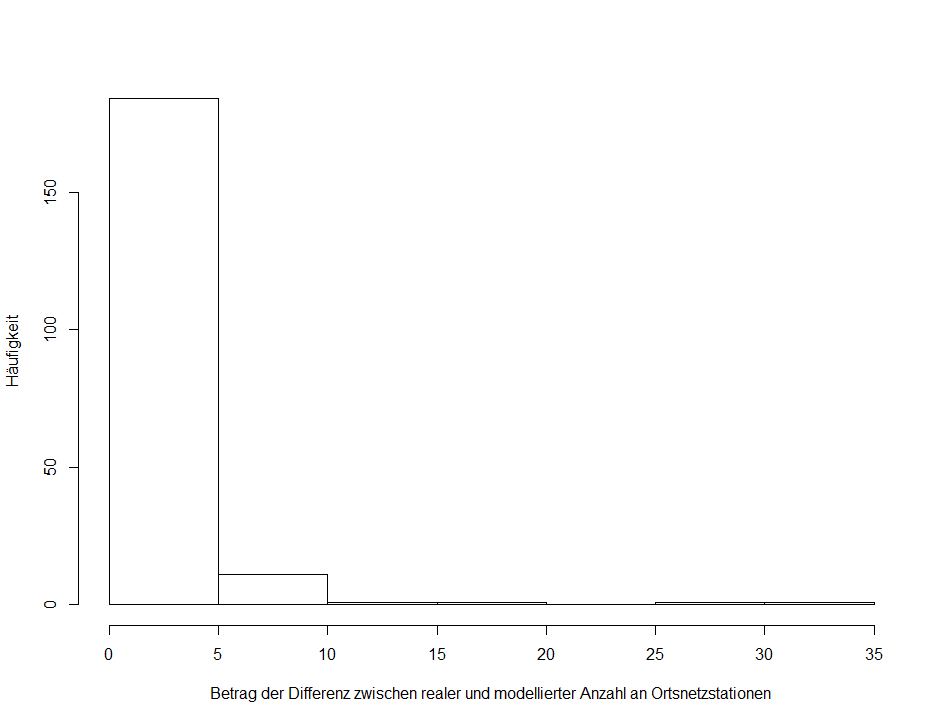
\includegraphics[keepaspectratio,width=0.8\textwidth,height=0.8\textheight]{bilder/hist_diff_abs}
\caption{Histogramm der Beträge der Unterschiede zwischen realer und modellierter Anzahl an Ortsnetzstationen\label{hist_diff_abs}}
\par\end{centering}

\end{figure}


Die Lagemaße dieser Verteilungen sind in  Tabelle \ref{tab:Lagemase_Unterschiede} zusammengefasst. 75\% der Werte liegen zwischen -2 und 1 beziehungsweise zwischen 0 und 2 Stationen Unterschied, es gibt jedoch Ausreißer, bei denen in der Modellierung bis zu 31 Ortsnetzstationen zu wenig erzeugt werden. 

\begin{table}
\caption{Lagemaße der Verteilung der Unterschiede zwischen den Anzahlen an Ortsnetzstationen\label{tab:Lagemase_Unterschiede}}

\noindent \centering{}%

\begin{tabular}{l|cccc}
 & Vorzeichen belassen & Betragswerte \tabularnewline
\hline 
Minimum & -10.00 & 0.00 \tabularnewline
Maximum & 31.00 & 31.00 \tabularnewline
1. Quantil & -2.00 & 0.00 \tabularnewline
Median & 0.00 & 1.00 \tabularnewline
3. Quantil & 1.00 & 2.00 \tabularnewline
Arithmetisches Mittel & -0.26 & 2.05 \tabularnewline
Standardabweichung & 4.29 & 3.77

\end{tabular}
\end{table}

Um mögliche Auswirkungen der Lastgebietsfläche auf den Modellfehler zu visualisieren, sind in den Abbildungen \ref{plot_area} und \ref{plot_area_abs} diese beiden Eigenschaften gegeneinander aufgetragen, \ref{plot_area_abs} bezieht sich hierbei wieder auf den absoluten Unterschied, während in  \ref{plot_area} Vorzeichen belassen worden sind.

\begin{figure}

\noindent \begin{centering}
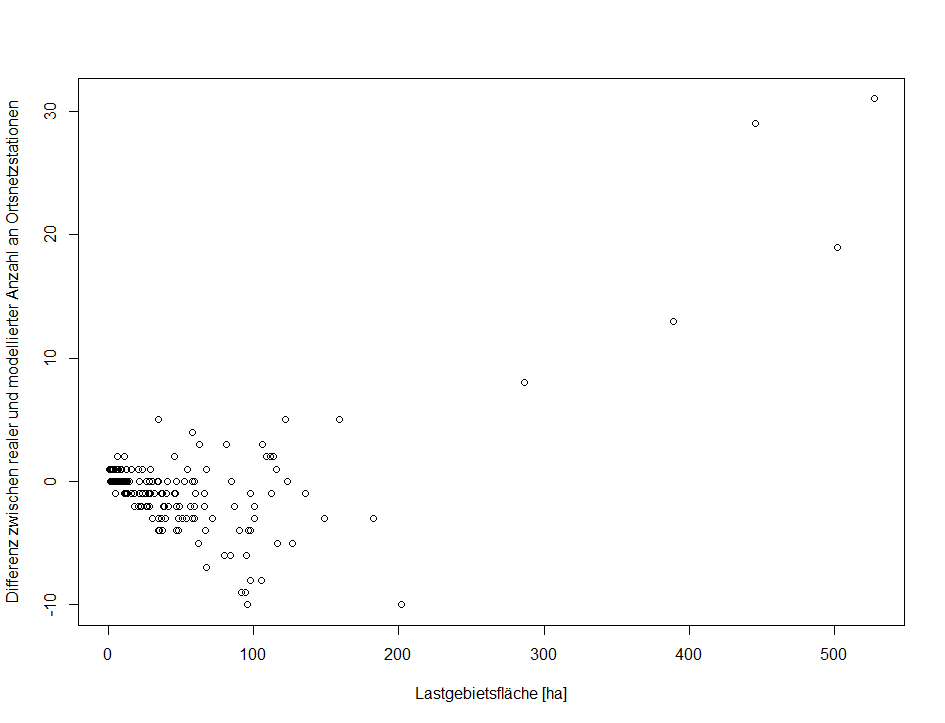
\includegraphics[keepaspectratio,width=0.8\textwidth,height=0.8\textheight]{bilder/plot_area}
\caption{Fläche der Lastgebiete und Unterschied zwischen realer und modellierter Anzahl an Ortsnetzstationen\label{plot_area}}
\par\end{centering}

\end{figure}

\begin{figure} 

\noindent \begin{centering}
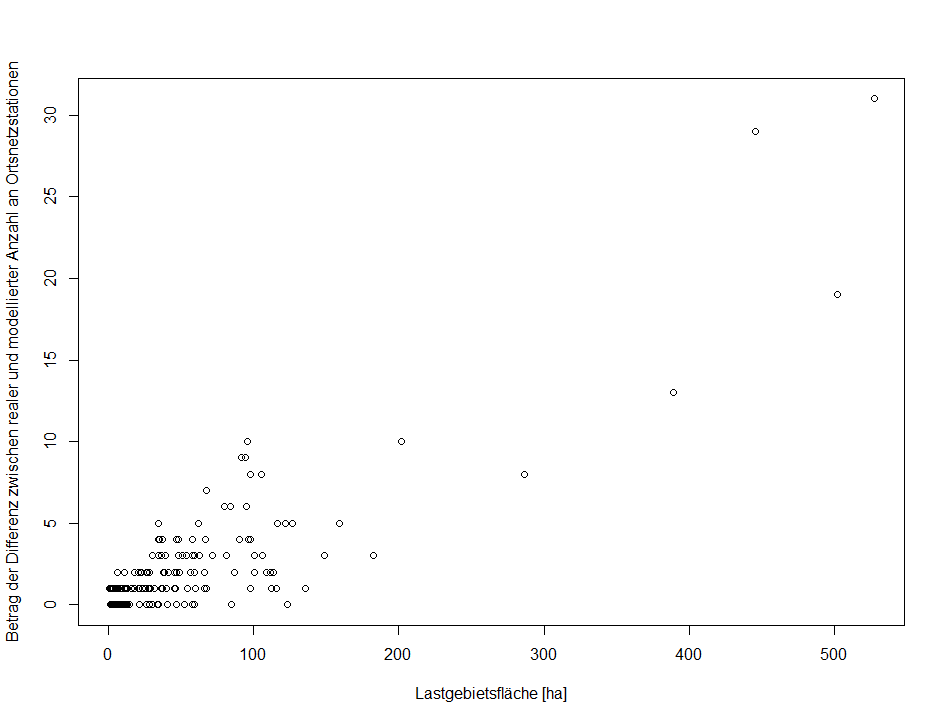
\includegraphics[keepaspectratio,width=0.8\textwidth,height=0.8\textheight]{bilder/plot_area_abs}
\caption{Fläche der Lastgebiete und Betrag der Differenz zwischen realer und modellierter Anzahl an Ortsnetzstationen\label{plot_area_abs}}
\par\end{centering}

\end{figure}

\newpage

\subsection{Position der Ortsnetzstationen}

Um die Lagegenauigkeit der modellierten Ortsnetzstationen zu bestimmen, wurde für jede modellierte Ortsnetzstation der Abstand zur nächstgelegenen realen Ortsnetzstation im jeweiligen Lastgebiet erhoben. Das Histogramm der Verteilung ist in Abbildung \ref{hist_dist_real_ons} zu sehen, die zugehörigen Lagemaße sind in Tabelle \ref{tab:dist_real_ons} dargestellt. Es ist zu erkennen, dass der Großteil der modellierten Ortsnetzstationen nicht weiter als 200 m von der nächstgelegenen realen Ortsnetzstation befindet, wobei einige Ausreißer bis in den Bereich von 1500 m zu beobachten sind.

\begin{figure} [b]

\noindent \begin{centering}
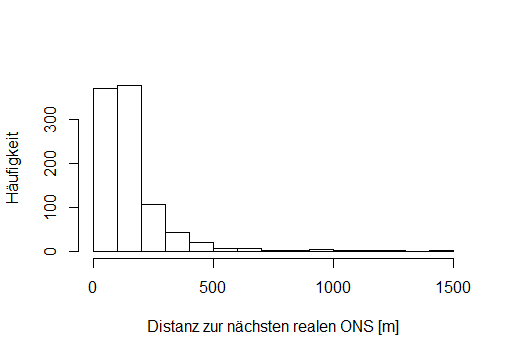
\includegraphics[keepaspectratio,width=0.8\textwidth,height=0.8\textheight]{bilder/hist_dist_real_ons}
\caption{Histogramm der Distanzen zur nächstgelegenen realen Ortsnetzstation\label{hist_dist_real_ons}}
\par\end{centering}

\end{figure}


\begin{table}[tbh]
\caption{Lagemaße der Verteilung der Distanz zur nächsten realen Ortsnetzstation\label{tab:dist_real_ons}}
\noindent \centering{}%

\begin{tabular}{l|cccc}

Minimum & 3.0  \tabularnewline
Maximum & 1479.0  \tabularnewline
1. Quantil & 76.0  \tabularnewline
Median & 120.5  \tabularnewline
3. Quantil & 179.2  \tabularnewline
Arithmetisches Mittel & 155.8  \tabularnewline
Standardabweichung & 4.29 

\end{tabular}
\end{table}

Um mögliche Auswirkungen der Lastgebietsfläche auf die Lagegenauigkeit zu visualisieren, sind in Abbildung \ref{plot_area_dist} diese beiden Eigenschaften gegeneinander aufgetragen. Der größte Teil der betrachteten Lastgebiete weist eine Fläche von weniger als 150 Hektar auf, lediglich in diesem Bereich befinden sich auch Ausreißer in der Lagegenauigkeit von bis etwa 600 m. Nur sehr wenige Lastgebiete überschreiten eine Fläche von 150 Hektar.

\begin{figure}

\noindent \begin{centering}
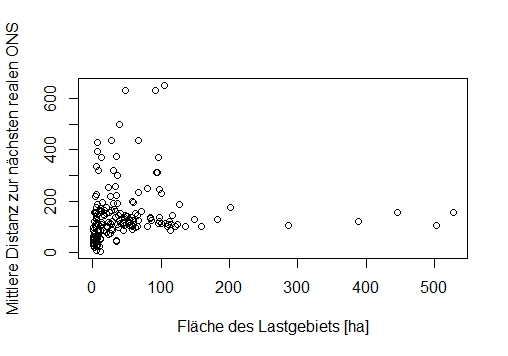
\includegraphics[keepaspectratio,width=0.8\textwidth,height=0.8\textheight]{bilder/plot_area_dist}
\caption{Lastgebietsflächen und mittlere Distanzen zur nächsten Ortsnetzstation\label{plot_area_dist}}
\par\end{centering}

\end{figure}

\chapter{Diskussion\label{chap:Diskussion} }

\section{Leitungen}

\subsection{Eignung von OpenStreetMap-Daten als Datenquelle des Straßennetzes}

Wie in Kapitel \ref{chap:Grundlagen} beschrieben, ist laut \citet{Neis2011} davon auszugehen, dass OpenStreetMap-Straßendaten in Deutschland seit 2012 eine mit kommerziellen Anbietern vergleichbare Vollständigkeit erreicht haben. Dies ist aber lediglich eine These, deren Richtigkeit wurde seitdem nicht überprüft. Auch ist die Vollständigkeit eines kommerziellen Datenanbieters nicht bekannt, sodass selbst bei Korrektheit von Neis' These noch eine unbekannte Anzahl von Straßen möglicherweise nicht in OpenStreetMap enthalten ist. Es lässt sich allerdings mit einiger Sicherheit sagen, dass, wenn der Vergleich mit einem kommerziellen Datenanbieter zutrifft, der Großteil der für Autonavigation zu gebrauchenden Straßen zur Verfügung steht und OpenStreetMap somit eine der vorliegenden Aufgabe angemessene Vollständigkeit bereitstellt.

Geht man davon aus, dass die Lagegenauigkeit von OpenStreetMap-Daten der Genauigkeit von GPS-Geräten entspricht, mit welchen ein großer Teil der Daten erhoben wurde, so ist eine Lagegenauigkeit zwischen 6 und 10 Metern zu erwarten \citep{Haklay2010}. für die vorliegende Fragestellung ist dies ausreichend. Wichtiger als die Lagegenauigkeit ist die Topologie des Straßennetzes, welche in OpenStreetMap als korrekt angenommen werden kann.

Schwierigkeiten bei der Nutzung von OpenStreetMap-Daten können allerdings durch die Attributgenauigkeit entstehen. Wie in Kapitel \ref{sec:Erstellung eines Netzdatensatzes aus OpenStreetMap-Strassendaten} beschrieben, wurden die zu betrachtenden Straßen auf Basis des "`highway"'-Schlüssels ausgewählt. Da die Attributierung in OpenStreetMap aber nur eine Richtlinie für die Mitglieder darstellt, kann es vorkommen, dass Straßen, die in die Auswahl aufgenommen werden sollten, auf andere Weise attributiert sind und somit übersehen werden. Auch besteht die Möglichkeit, dass Objekte fälschlicherweise mit einem "`highway"'-Wert attributiert sind, obwohl sie etwas anderes darstellen sollen. Hier macht sich das generelle Risiko in der Nutzung von VGI-Daten bemerkbar, welches in dem Fehlen einer zentralen Kontrollinstanz besteht, die unter anderem die Homogenität der Metadaten garantiert.


\subsection{Eignung des Straßennetzes zur Abbildung von Niederspannungsnetzen}

Die Grundüberlegung der vorliegenden Arbeit besteht darin, dass Niederspannungsleitungen in der Regel unter Straßen verlegt sind, und das Straßennetz daher zur Abbildung des Niederspannungsnetzes geeignet ist. Selbst bei einem komplett fehlerfreiem Straßendatensatz gibt es hier allerdings Einschränkungen. Zum Einen gilt die obige Überlegung lediglich für unterirdisch verlegte Kabel. Oberirdische Freileitungen können nach anderen Gesichtspunkten verlegt sein und vom Straßenverlauf abweichen. Freileitungen machen jedoch in den meisten Gebieten nur einen geringen Anteil des Gesamtnetzes aus, unter den zur Validierung genutzten Gebieten betrug der höchste Anteil an Freileitungen etwa 15 \%. Die Bedeutung von Freileitungen in der Niederspannung wird in Zukunft weiter zurückgehen, da Niederspannungsnetze heutzutage als Kabelnetze geplant werden \citep{Heuck2013}.

Weiterhin gilt der Umstand, dass Kabel in der Regel dem Straßenverlauf folgen, sicherlich nicht ohne Ausnahme. Es kann Einzelfälle geben, in denen die Kabelverlegung unter einer Straße nicht sinnvoll ist, darüber hinaus gibt es natürlich auch Straßen, unter denen keine Niederspannungskabel verlegt sind. Diese Fälle können von der verwendeten Methode nicht abgefangen werden. Da nicht bekannt ist, in welchem Ausmaß Abweichungen von der genannten Regel vorhanden sind, müsste dies durch eine geeignete Validierung erhoben werden, näheres dazu im Kapitel \ref{Validierungsprozess}.

Schließlich kann das Straßennetz nur Informationen über den Verlauf der Kabel, nicht aber über deren Anzahl wiedergeben. Diese ist aber wichtig für elektrotechnische Betrachtungen. Unter einer Straße können entweder beidseitig oder nur auf einer Seite Kabel verlaufen \citep{Heuck2013}, was allein durch Betrachtung der Straße nicht ersichtlich ist. Indikatoren dafür könnte beispielsweise die Bebauung liefern: In dicht bebauten Gebieten, in denen beidseitig der Straße Gebäude stehen, ist die Wahrscheinlichkeit höher, dass auch auf beiden Seiten der Straße Kabel verlegt sind. Da die Bebauung aufgrund der unbekannten, vermutlich mangelhaften, Vollständigkeit in OpenStreetMap nicht für die vorliegende Arbeit genutzt wurde, kann hierzu noch keine Aussage getroffen werden.

\subsection{Validierungsprozess\label{Validierungsprozess}}

Der hier verwendete Validierungsprozess, in dem die Leitungslängen des Niederspannungsnetzes für bestimmte Netzbetreibergebiete mit den in diesen Gebieten erhobenen Straßenlängen verglichen wurden, stellt lediglich eine behelfsmäßige Methode dar, die aus dem Mangel an geeigneten Validierungsdaten entstand. Anders als für die Ortsnetzstationen stand für das Kabelnetz kein flächendeckender Datensatz zur Verfügung, mit Ausnahme des Niederspannungsnetzes der Ortschaft Tussenhausen, das alleine nicht für eine Validierung ausreichend ist. Somit kann keine Aussage über die Lagegenauigkeit der erzeugten künstlichen Netze gemacht werden. Dafür wäre ein entsprechender Datensatz notwendig.
Die Kabellängen können mit den Straßenlängen in den in Kapitel \ref{Validierung} genannten Gebieten verglichen werden, allerdings sind diese Längen auf sehr großen Flächen von rund 1000 km$^2$ aggregiert. Auf der Ebene der Lastgebiete könnten andere Ergebnisse vorliegen, die von der Aggregierung überdeckt werden. Auch die vorliegenden Daten lassen jedoch schon einen klaren Unterschied zwischen Straßen- und Leitungslängen erkennen. Ein plausibler Grund für den Fehlbetrag von 1,05 Kilometern pro Quadratkilometer ist die zu vermutende beidseitige Verkabelung von Straßen. Dadurch beträgt die Leitungslänge in den entsprechenden Straßenabschnitten das Doppelte der Straßenlänge, was den insgesamt deutlich kleineren Wert der Straßenlängen erklärt. Letztlich belegen lässt sich dies jedoch wiederum nur mit einem geeigneten Validierungsdatensatz.

Bei der Betrachtung der Flächen der Validierungsgebiete ist zu beachten, dass der Flächenbegriff möglicherweise von den Netzbetreibern unterschiedlich ausgelegt wird. Manche Netzbetreiber geben sowohl eine geographische Fläche, als auch eine versorgte Fläche ihres Netzgebiets an, wobei die versorgte Fläche lediglich die Gebiete bezeichnet, in denen Strom verbraucht wird. In der geographischen Fläche sind auch unbebaute Gebiete eingeschlossen, die innerhalb der Gemarkung der versorgten Ortschaften liegen. für eines der als Validierungsgebiete ausgewählten Netzgebiete wurde in den Angaben des Netzbetreibers die geographische Fläche nach Spannungsebenen gegliedert, für die übrigen beiden wurde nur ein einzelner Wert für die geographische Fläche angegeben. Es besteht die Möglichkeit, dass die auf die Netzgebietsflächen bezogene Abweichung zwischen Straßen- und Leitungslängen deswegen verfälscht ist. Auch ohne Flächenbezug ist aber ein deutlicher Unterschied zu erkennen, sodass eine etwaige Verzerrung dieses Wertes nichts an der Aussage des Ergebnisses ändert.


\section{Ortsnetzstationen}

\subsection{Einzugsgebiete der Ortsnetzstationen}

Die Angaben zur Größe der Einzugsgebiete, die zur Bestimmung der Anzahl an Ortsnetzstationen verwendet werden, beziehen sich, wie in Kapitel \ref{Modellierung der Ortsnetzstationen} erwähnt, auf Siedlungen niedriger Dichte. Die vorgestellte Methode zur Erzeugung künstlicher Ortsnetzstationen sollte daher nur auf Gebiete angewandt werden, auf die diese Bezeichnung zutrifft.
Weiterhin ist zu beachten, dass diese Angaben lediglich Durchschnittswerte sind, manche Lastgebiete können stark davon abweichen.
Außerdem wurde das Verhältnis zwischen der Länge einer Niederspannungsleitung und der Luftlinienentfernung von deren Start- zu deren Endpunkt, das ebenfalls zur Konzipierung der Einzugsgebietsgrößen verwendet wurde, empirisch aufgrund von Erhebungen in der Ortschaft Tussenhausen im Untersuchungsgebiet bestimmt. Die Werte von Tussenhausen müssen nicht notwendigerweise repräsentativ für das gesamte Untersuchungsgebiet sein und sind somit nicht optimal, liefern aber die beste verfügbare Annäherung an die Werte der Grundgesamtheit. Wie schon im vorigen Abschnitt gilt auch hier die Einschränkung, dass es sich um einen Mittelwert handelt, von dem manche Lastgebiete unter Umständen abweichen können. 

Da bei der in Kapitel \ref{Modellierung der Ortsnetzstationen} beschriebenen Methode nur Gittermittelpunkte als Ortsnetzstationen gezählt werden, die sich innerhalb des jeweiligen Lastgebiets befinden, kann die Form des Lastgebiets einen starken Einfluss auf die kalkulierte Anzahl der Ortsnetzstationen haben, wobei dies durch den zweiten Schritt, in dem nachträglich Ortsnetzstationen hinzugefügt werden, gedämpft wird.

Die Diskrepanz zwischen realen und modellierten Ortsnetzstationen ist mit 11,76 \% trotz der genannten Einschränkungen recht gering, was dafür spricht, dass die gemachten Annahmen der Realität nahekommen. Die Anzahl der realen Ortsnetzstationen ist außerdem etwas nach oben verfälscht, da in dem ursprünglich vorliegenden SINCAL-Format manche Ortsnetzstationen aus mehreren Objekten bestanden, und diese Mehrfachnennung beim Import in die Datenbank übernommen wurde. 

Auf Ebene der einzelnen Lastgebiete ist die mittlere Diskrepanz von etwa zwei Ortsnetzstationen trotzdem einschneidend, wenn man bedenkt, dass der Großteil der betrachteten Lastgebiete mit weniger als 150 Hektar recht klein ist und daher vermutlich sowieso nur wenige Ortsnetzstationen beinhaltet.

\subsection{Position der Ortsnetzstationen}

Unter den gefundenen Prediktoren, die mit Hilfe der Stepwise Variable Selection ausgewählt wurden, um die Wahrscheinlichkeit des Vorhandenseins einer Ortsnetzstation zu bestimmen, befinden sich unter anderem die Variablen "`Bevölkerung im Umkreis von 50 m"' und "`Bevölkerung im Umkreis von 100 m"'. Die Koeffizienten dieser Variablen haben unterschiedliche Vorzeichen, obwohl beide sehr ähnliche Eigenschaften beschreiben. Es ist unwahrscheinlich, dass die Bevölkerungszahl innerhalb von 50 Metern sich positiv, innerhalb von 100 Metern aber negativ auf die Wahrscheinlichkeit des Vorhandenseins einer Ortsnetzstation auswirkt, daher besteht vermutlich ein Fehler in der Variablenauswahl. Vermutlich war der zur Bestimmung der Kollinearität verwendete Varianzinflationsfaktor nicht ausreichend, um alle korrelierten Variablen auszusieben. Die Koeffizienten der restlichen Variablen entsprechen den Erwartungen: Hohe Distanzen zu Straßen und Straßenkreuzungen führen zu niedriger, Hohe Gebäudeanzahlen und Gebäudeflächen zu erhöhter Wahrscheinlichkeit des Auftretens von Ortsnetzstationen.

Die Validierung der Lage der modellierten Ortsnetzstationen zeigt, dass der Median des Abstands zur nächsten realen Ortsnetzstation bei 120 Metern liegt. Da ein durchschnittlicher Niederspannungsstrang selbst aber nur 200-300 Meter lang ist, ist dies kein sehr genauer Wert. Die Position der Ortsnetzstationen wird durch die verwendete Methode also nur unzureichend abgebildet. 

Eine weitere Unsicherheit besteht darin, dass die vom Netzbetreiber LVN bereitgestellten Daten über keine Informationen zur Lagegenauigkeit verfügen. Ein visueller Vergleich mit OpenStreetMap-Kartenausschnitten der Ortschaft Tussenhausen im Untersuchungsgebiet und der dort verfügbaren Leitungsdaten legt jedoch eine Lagegenauigkeit im einstelligen Meterbereich nahe.

\subsection{Einfluss der Lastgebietsfläche auf die Ergebnisse}

Die Gegenüberstellung von Lastgebietsfläche und der Diskrepanz zwischen realer und modellierter Anzahl an Ortsnetzstationen in Abbildung \ref{plot_area_abs} 
lässt vermuten, dass ein Zusammenhang zwischen Größe des Lastgebiets und Ausmaß der Diskrepanz vorliegt. Dies ist nicht verwunderlich, da kleine Lastgebiete wenig Spielraum für Fehler lassen, dagegen kann die Form und Bebauungsdichte in größeren Lastgebieten zu stark variierenden Ergebnissen führen.

Betrachtet man die Fläche der Lastgebiete im Bezug zur Lagegenauigkeit, die in Abbildung \ref{plot_area_dist} als mittlere Distanz der modellierten Ortsnetzstationen zur nächstgelegenen realen Ortsnetzstation dargestellt ist, ist auf den ersten Blick keine Abhängigkeit zu erkennen. Zwar ist eine scheinbar abnehmende Distanz mit zunehmender Lastgebietsfläche erkennbar, allerdings nicht in den Bereichen, in denen ausreichend Datenpunkte vorhanden sind, um dies zu belegen. Somit wird davon ausgegangen, dass die Fläche des Lastgebiets bei Anwendung der hier vorgestellten Methode keine Rolle für die Lagegenauigkeit des Ergebnisses spielt.


\subsection{}
Ausreißer bei Validierung (Regression) diskutieren





\chapter{Fazit\label{chap:Fazit} }

Das Ziel der vorliegenden Arbeit bestand in der Abbildung von deutschen Niederspannungsnetzen. Die daraus resultierenden künstlichen Netze sollten etwa dazu verwendet werden können, die Kosten des zukünftigen Netzausbaus im Niederspannungsbereich abzuschätzen. Für den ersten Teil dieser Aufgabe, die Erzeugung von künstlichen Leitungsdaten aus OpenStreetMap, besteht die größte Schwierigkeit im Mangel an Validierungsdaten. Die erzeugten Netzformen konnten hinsichtlich des Leitungsverlaufs nicht validiert werden, weil geeignete Datensätze zur Validierung nicht zur Verfügung standen. Die Validierung der Leitungslängen, die aggregiert auf die Netzgebiete verschiedener Netzbetreiber vorgenommen wurde, lässt aber bereits erkennen, dass mit der verwendeten Methode zu wenige Leitungen erzeugt wurden. Dies muss nicht notwendigerweise darauf hindeuten, dass Straßen nicht ausreichend für die Abbildung von Niederspannungsnetzen sind: Eine wahrscheinliche Ursache für die Längen-Diskrepanz liegt in dem Umstand, dass Niederspannungskabel in manchen Fällen auf beiden Seiten einer Straße verlegt sind, und die Länge mancher Straßenabschnitte somit nur halb so groß wie die Länge der darunter verlaufenden Leitungen ist. Um dies zu prüfen, sind wiederum geeignete Leitungsdaten zur Validierung notwendig.
Der zweite Teil der Arbeit, die Erzeugung künstlicher Ortsnetzstationen, weist gute Ergebnisse im Hinblick auf die Anzahl der Ortsnetzstationen pro Lastgebiet auf. Die mit Hilfe einer Stepwise Variable Selection und einer logistischen Regression sowie eines graphentheoretischen Algorithmus ausgewählten Standorte der Ortsnetzstationen bilden jedoch nicht die tatsächlichen Lagen der realen Ortsnetzstationen ab, wie der Vergleich beider Datensätze zeigt. Da es aber bei elektrotechnischen Betrachtungen weniger auf die genaue Lage der Betriebsmittel, als vielmehr auf die topologischen Eigenschaften und die Abstände zwischen den Objekten ankommt, kann das Ergebnis unter Umständen immer noch für manche Zwecke genutzt werden.
Zusammenfassend lässt sich somit sagen, dass zwar die genaue Abbildung der realen Netze nicht gelungen ist, jedoch der Zweck - Modellnetze zu erstellen, die sich in der elektrotechnischen Betrachtung möglichst ähnlich den realen Netzen verhalten - möglicherweise trotzdem erfüllt werden kann. Allerdings sind dafür neben den für Anwendungen außerhalb des Untersuchungsgebiets benötigten Datenerhebungen vor allem eine genauere Validierung der erzeugten Netzdaten notwendig. Zu möglichen zukünftigen Untersuchungen, die an die Ergebnisse der vorliegenden Arbeit anschließen, gehört daher an erster Stelle die erwähnte Validierung. Außerdem wichtig sind das Erkennen von Straßenabschnitten mit beidseitiger Kabelverlegung, eventuell über die anliegende Bebauung, sowie Untersuchungen zum elektrotechnischen Verhalten der erzeugten Netze.

\clearpage{}

\bibliographystyle{bibtex/dinat_mod}
\phantomsection\addcontentsline{toc}{chapter}{\bibname}\bibliography{bibtex/MA_Arbeit_Guetter_Literatur}


\appendix
\appendixpage


\chapter{Plots zur Datenexploration im Vorfeld der logistischen Regression\label{chap:Plots zur Datenexploration im Vorfeld der logistischen Regression}}

\begin{figure}[ht]
\minibox[frame]{
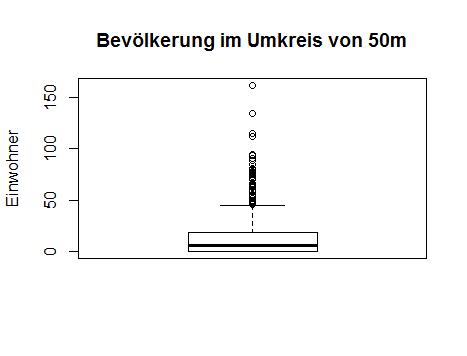
\includegraphics[keepaspectratio,width=\textwidth/2,height=\textheight/2]{bilder/Anhang_A/boxplot1}
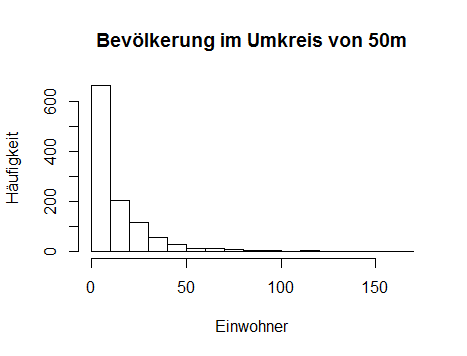
\includegraphics[keepaspectratio,width=\textwidth/2,height=\textheight/2]{bilder/Anhang_A/hist1} \\
\parbox [b][3.7cm][t]{\textwidth/2}
	{
	\qquad Arithmetisches Mittel: 12.39 
			
	\qquad Minimum: 0.00
	
	\qquad Maximum: 162.00
	
	\qquad 1. Quantil: 0.00
	
	\qquad Median: 6.00
	
	\qquad 3. Quantil: 18.00
	
	}
\includegraphics[keepaspectratio,width=\textwidth/2,height=\textheight/2,clip = true]{bilder/Anhang_A/spine1}
}
\end{figure}

\begin{figure}[ht]
\minibox[frame]{
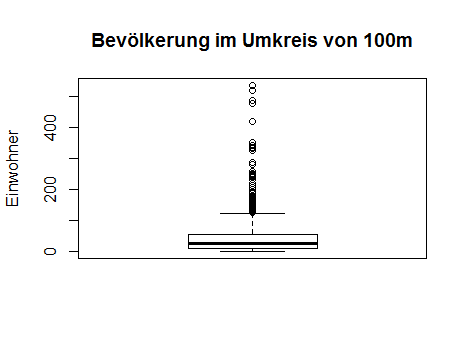
\includegraphics[keepaspectratio,width=\textwidth/2,height=\textheight/2]{bilder/Anhang_A/boxplot2}
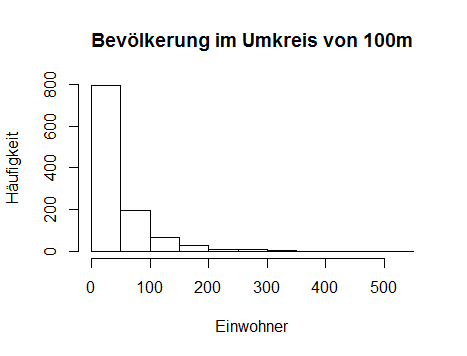
\includegraphics[keepaspectratio,width=\textwidth/2,height=\textheight/2]{bilder/Anhang_A/hist2} \\
\parbox [b][3.7cm][t]{\textwidth/2}
	{
	\qquad Arithmetisches Mittel: 44.36 
			
	\qquad Minimum: 0.00
	
	\qquad Maximum: 537.00
	
	\qquad 1. Quantil: 8.00
	
	\qquad Median:27.00
	
	\qquad 3. Quantil: 55.00
	
	}
\includegraphics[keepaspectratio,width=\textwidth/2,height=\textheight/2,clip = true]{bilder/Anhang_A/spine2}
}
\end{figure}

\begin{figure}[ht]
\minibox[frame]{
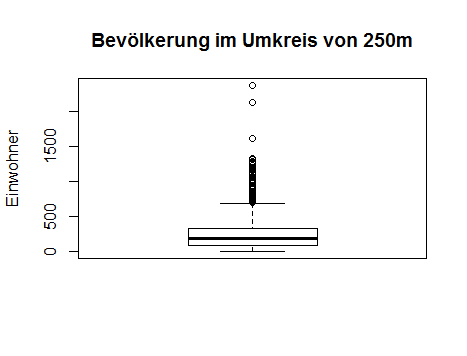
\includegraphics[keepaspectratio,width=\textwidth/2,height=\textheight/2]{bilder/Anhang_A/boxplot3}
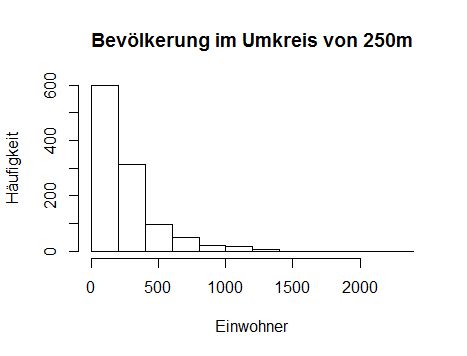
\includegraphics[keepaspectratio,width=\textwidth/2,height=\textheight/2]{bilder/Anhang_A/hist3} \\
\parbox [b][3.7cm][t]{\textwidth/2}
	{
	\qquad Arithmetisches Mittel: 254.7 
			
	\qquad Minimum: 0.0
	
	\qquad Maximum: 2372.0
	
	\qquad 1. Quantil: 86.0
	
	\qquad Median: 185.0
	
	\qquad 3. Quantil: 328.0
	
	}
\includegraphics[keepaspectratio,width=\textwidth/2,height=\textheight/2,clip = true]{bilder/Anhang_A/spine3}
}
\end{figure}

\begin{figure}[ht]
\minibox[frame]{
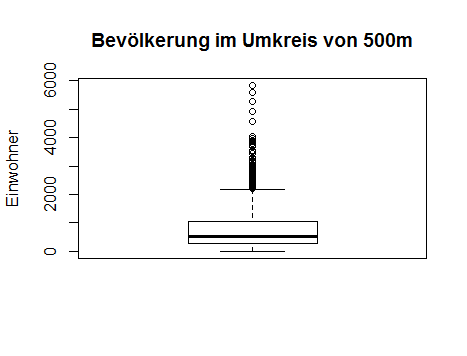
\includegraphics[keepaspectratio,width=\textwidth/2,height=\textheight/2]{bilder/Anhang_A/boxplot4}
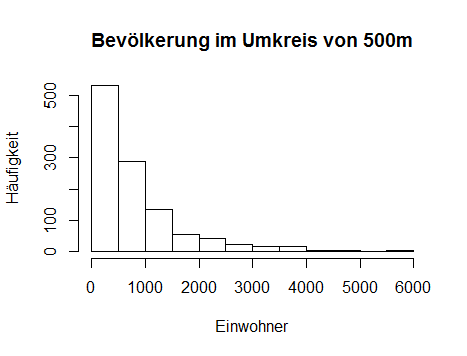
\includegraphics[keepaspectratio,width=\textwidth/2,height=\textheight/2]{bilder/Anhang_A/hist4} \\
\parbox [b][3.7cm][t]{\textwidth/2}
	{
	\qquad Arithmetisches Mittel: 815.2 
			
	\qquad Minimum: 0.0
	
	\qquad Maximum: 5837.0
	
	\qquad 1. Quantil: 275.0
	
	\qquad Median: 530.0
	
	\qquad 3. Quantil: 1042.0
	
	}
\includegraphics[keepaspectratio,width=\textwidth/2,height=\textheight/2,clip = true]{bilder/Anhang_A/spine4}
}
\end{figure}

\begin{figure}[ht]
\minibox[frame]{
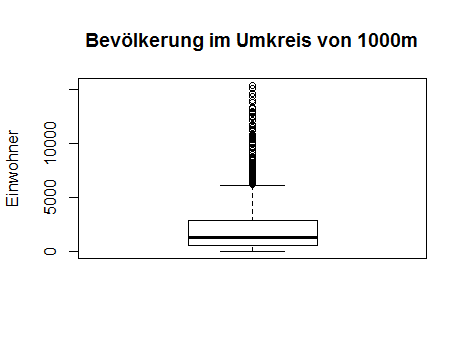
\includegraphics[keepaspectratio,width=\textwidth/2,height=\textheight/2]{bilder/Anhang_A/boxplot5}
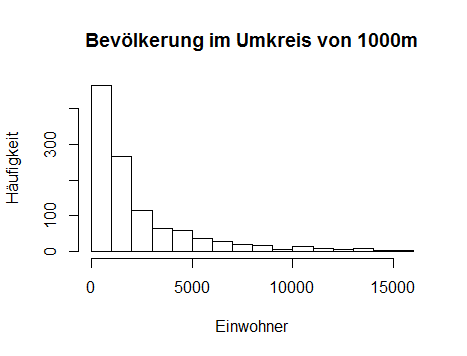
\includegraphics[keepaspectratio,width=\textwidth/2,height=\textheight/2]{bilder/Anhang_A/hist5} \\
\parbox [b][3.7cm][t]{\textwidth/2}
	{
	\qquad Arithmetisches Mittel: 2294 
			
	\qquad Minimum: 0
	
	\qquad Maximum: 15350
	
	\qquad 1. Quantil: 592
	
	\qquad Median: 1262
	
	\qquad 3. Quantil: 2830
	
	}
\includegraphics[keepaspectratio,width=\textwidth/2,height=\textheight/2,clip = true]{bilder/Anhang_A/spine5}
}
\end{figure}

\begin{figure}[ht]
\minibox[frame]{
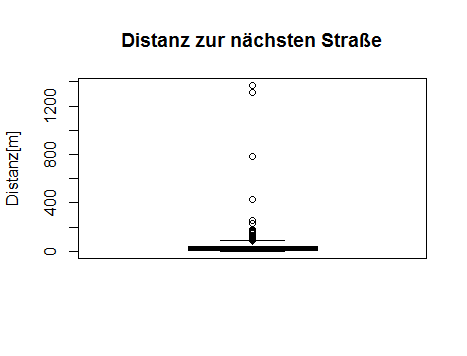
\includegraphics[keepaspectratio,width=\textwidth/2,height=\textheight/2]{bilder/Anhang_A/boxplot6}
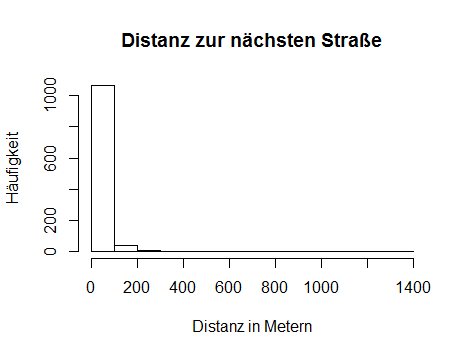
\includegraphics[keepaspectratio,width=\textwidth/2,height=\textheight/2]{bilder/Anhang_A/hist6} \\
\parbox [b][3.7cm][t]{\textwidth/2}
	{
	\qquad Arithmetisches Mittel: 33.95 
			
	\qquad Minimum: 0.00
	
	\qquad Maximum: 1371.00
	
	\qquad 1. Quantil: 9.00
	
	\qquad Median: 21.00
	
	\qquad 3. Quantil: 42.00
	
	}
\includegraphics[keepaspectratio,width=\textwidth/2,height=\textheight/2,clip = true]{bilder/Anhang_A/spine6}
}
\end{figure}

\begin{figure}[ht]
\minibox[frame]{
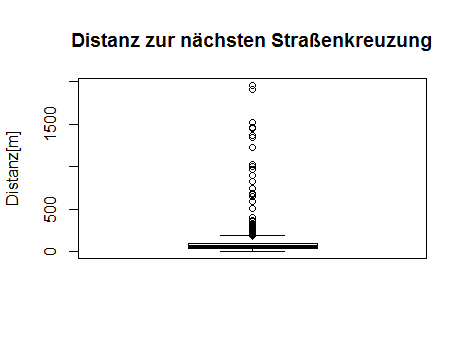
\includegraphics[keepaspectratio,width=\textwidth/2,height=\textheight/2]{bilder/Anhang_A/boxplot7}
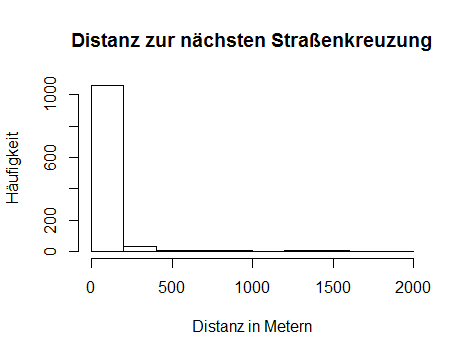
\includegraphics[keepaspectratio,width=\textwidth/2,height=\textheight/2]{bilder/Anhang_A/hist7} \\
\parbox [b][3.7cm][t]{\textwidth/2}
	{
	\qquad Arithmetisches Mittel: 87.93 
			
	\qquad Minimum: 1.00
	
	\qquad Maximum: 1956.00
	
	\qquad 1. Quantil: 33.00
	
	\qquad Median: 59.00
	
	\qquad 3. Quantil: 96.00
	
	}
\includegraphics[keepaspectratio,width=\textwidth/2,height=\textheight/2,clip = true]{bilder/Anhang_A/spine7}
}
\end{figure}

\begin{figure}[ht]
\minibox[frame]{
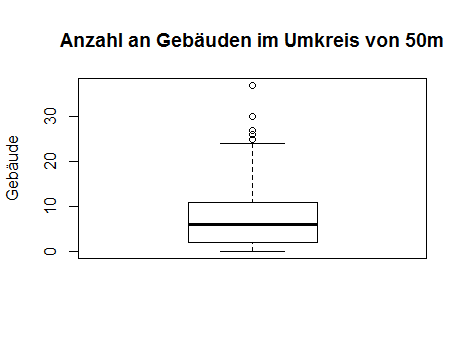
\includegraphics[keepaspectratio,width=\textwidth/2,height=\textheight/2]{bilder/Anhang_A/boxplot8}
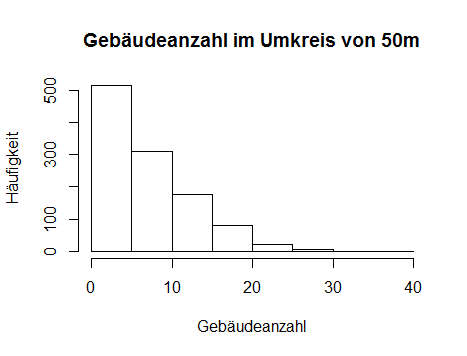
\includegraphics[keepaspectratio,width=\textwidth/2,height=\textheight/2]{bilder/Anhang_A/hist8} \\
\parbox [b][3.7cm][t]{\textwidth/2}
	{
	\qquad Arithmetisches Mittel: 7.156 
			
	\qquad Minimum: 0.000
	
	\qquad Maximum: 37.000
	
	\qquad 1. Quantil: 2.000
	
	\qquad Median: 6.000
	
	\qquad 3. Quantil: 11.000
	
	}
\includegraphics[keepaspectratio,width=\textwidth/2,height=\textheight/2,clip = true]{bilder/Anhang_A/spine8}
}
\end{figure}

\begin{figure}[ht]
\minibox[frame]{
\includegraphics[keepaspectratio,width=\textwidth/2,height=\textheight/2]{bilder/Anhang_A/boxplot9}
\includegraphics[keepaspectratio,width=\textwidth/2,height=\textheight/2]{bilder/Anhang_A/hist9} \\
\parbox [b][3.7cm][t]{\textwidth/2}
	{
	\qquad Arithmetisches Mittel: 23.03 
			
	\qquad Minimum: 0.00
	
	\qquad Maximum: 95.00
	
	\qquad 1. Quantil: 8.00
	
	\qquad Median: 19.00
	
	\qquad 3. Quantil: 34.00
	
	}
\includegraphics[keepaspectratio,width=\textwidth/2,height=\textheight/2,clip = true]{bilder/Anhang_A/spine9}
}
\end{figure}

\begin{figure}[ht]
\minibox[frame]{
\includegraphics[keepaspectratio,width=\textwidth/2,height=\textheight/2]{bilder/Anhang_A/boxplot10}
\includegraphics[keepaspectratio,width=\textwidth/2,height=\textheight/2]{bilder/Anhang_A/hist10} \\
\parbox [b][3.7cm][t]{\textwidth/2}
	{
	\qquad Arithmetisches Mittel: 107.9 
			
	\qquad Minimum: 0.0
	
	\qquad Maximum: 410.0
	
	\qquad 1. Quantil: 48.0
	
	\qquad Median: 93.0
	
	\qquad 3. Quantil: 158.0
	
	}
\includegraphics[keepaspectratio,width=\textwidth/2,height=\textheight/2,clip = true]{bilder/Anhang_A/spine10}
}
\end{figure}

\begin{figure}[ht]
\minibox[frame]{
\includegraphics[keepaspectratio,width=\textwidth/2,height=\textheight/2]{bilder/Anhang_A/boxplot11}
\includegraphics[keepaspectratio,width=\textwidth/2,height=\textheight/2]{bilder/Anhang_A/hist11} \\
\parbox [b][3.7cm][t]{\textwidth/2}
	{
	\qquad Arithmetisches Mittel: 326.9 
			
	\qquad Minimum: 0.0
	
	\qquad Maximum: 1136.0
	
	\qquad 1. Quantil: 150.0
	
	\qquad Median: 286.0
	
	\qquad 3. Quantil: 458.0
	
	}
\includegraphics[keepaspectratio,width=\textwidth/2,height=\textheight/2,clip = true]{bilder/Anhang_A/spine11}
}
\end{figure}

\begin{figure}[ht]
\minibox[frame]{
\includegraphics[keepaspectratio,width=\textwidth/2,height=\textheight/2]{bilder/Anhang_A/boxplot12}
\includegraphics[keepaspectratio,width=\textwidth/2,height=\textheight/2]{bilder/Anhang_A/hist12} \\
\parbox [b][3.7cm][t]{\textwidth/2}
	{
	\qquad Arithmetisches Mittel: 831.2 
			
	\qquad Minimum: 0.0
	
	\qquad Maximum: 2948.0
	
	\qquad 1. Quantil: 329.0
	
	\qquad Median: 674.0
	
	\qquad 3. Quantil: 1120.0
	
	}
\includegraphics[keepaspectratio,width=\textwidth/2,height=\textheight/2,clip = true]{bilder/Anhang_A/spine12}
}
\end{figure}

\begin{figure}[ht]
\minibox[frame]{
\includegraphics[keepaspectratio,width=\textwidth/2,height=\textheight/2]{bilder/Anhang_A/boxplot13}
\includegraphics[keepaspectratio,width=\textwidth/2,height=\textheight/2]{bilder/Anhang_A/hist13} \\
\parbox [b][3.7cm][t]{\textwidth/2}
	{
	\qquad Arithmetisches Mittel: 3029 
			
	\qquad Minimum: 0.0
	
	\qquad Maximum: 90090.0
	
	\qquad 1. Quantil: 833.5
	
	\qquad Median: 1841.0
	
	\qquad 3. Quantil: 2972.0
	
	}
\includegraphics[keepaspectratio,width=\textwidth/2,height=\textheight/2,clip = true]{bilder/Anhang_A/spine13}
}
\end{figure}

\begin{figure}[ht]
\minibox[frame]{
\includegraphics[keepaspectratio,width=\textwidth/2,height=\textheight/2]{bilder/Anhang_A/boxplot14}
\includegraphics[keepaspectratio,width=\textwidth/2,height=\textheight/2]{bilder/Anhang_A/hist14} \\
\parbox [b][3.7cm][t]{\textwidth/2}
	{
	\qquad Arithmetisches Mittel: 7169 
			
	\qquad Minimum: 0
	
	\qquad Maximum: 95650
	
	\qquad 1. Quantil: 3194
	
	\qquad Median: 5977
	
	\qquad 3. Quantil: 8477
	
	}
\includegraphics[keepaspectratio,width=\textwidth/2,height=\textheight/2,clip = true]{bilder/Anhang_A/spine14}
}
\end{figure}

\begin{figure}[ht]
\minibox[frame]{
\includegraphics[keepaspectratio,width=\textwidth/2,height=\textheight/2]{bilder/Anhang_A/boxplot15}
\includegraphics[keepaspectratio,width=\textwidth/2,height=\textheight/2]{bilder/Anhang_A/hist15} \\
\parbox [b][3.7cm][t]{\textwidth/2}
	{
	\qquad Arithmetisches Mittel: 28210 
			
	\qquad Minimum: 0
	
	\qquad Maximum: 153800
	
	\qquad 1. Quantil: 14160
	
	\qquad Median: 24590
	
	\qquad 3. Quantil: 38040
	
	}
\includegraphics[keepaspectratio,width=\textwidth/2,height=\textheight/2,clip = true]{bilder/Anhang_A/spine15}
}
\end{figure}

\begin{figure}[ht]
\minibox[frame]{
\includegraphics[keepaspectratio,width=\textwidth/2,height=\textheight/2]{bilder/Anhang_A/boxplot16}
\includegraphics[keepaspectratio,width=\textwidth/2,height=\textheight/2]{bilder/Anhang_A/hist16} \\
\parbox [b][3.7cm][t]{\textwidth/2}
	{
	\qquad Arithmetisches Mittel: 80020 
			
	\qquad Minimum: 0
	
	\qquad Maximum: 264400
	
	\qquad 1. Quantil: 39160
	
	\qquad Median: 67000
	
	\qquad 3. Quantil: 111700
	
	}
\includegraphics[keepaspectratio,width=\textwidth/2,height=\textheight/2,clip = true]{bilder/Anhang_A/spine16}
}
\end{figure}

\begin{figure}[ht]
\minibox[frame]{
\includegraphics[keepaspectratio,width=\textwidth/2,height=\textheight/2]{bilder/Anhang_A/boxplot17}
\includegraphics[keepaspectratio,width=\textwidth/2,height=\textheight/2]{bilder/Anhang_A/hist17} \\
\parbox [b][3.7cm][t]{\textwidth/2}
	{
	\qquad Arithmetisches Mittel: 205600 
			
	\qquad Minimum: 0
	
	\qquad Maximum: 774500
	
	\qquad 1. Quantil: 72500
	
	\qquad Median: 148500
	
	\qquad 3. Quantil: 294400
	
	}
\includegraphics[keepaspectratio,width=\textwidth/2,height=\textheight/2,clip = true]{bilder/Anhang_A/spine17}
}
\end{figure}

\chapter{SQL-Code zur Netzgenerierung aus OpenStreetMap-Straßendaten\label{chap:SQL-Code zur Netzgenerierung aus OpenStreetMap-Straßendaten}}

\lstinputlisting  [language=SQL,tabsize=1,breaklines=true]{Quellcode/strassen.sql}

\chapter{SQL-Code zur Erhebung potentieller Prediktoren\label{chap:SQL-Code zur Erhebung potentieller Prediktoren}}

\lstinputlisting  [language=SQL,tabsize=1,breaklines=true]{Quellcode/candidatpoints.sql}

\chapter{R-Code zur logistischen Regression\label{chap:R-Code zur logistischen Regression}}

\lstinputlisting  [language=R,tabsize=1,breaklines=true]{Quellcode/logistische_regression.R}

\chapter{Python-Code zur Positionierung von Ortsnetzstationen\label{chap:Python-Code zur Positionierung von Ortsnetzstationen}}

\lstinputlisting  [language=Python,tabsize=1,breaklines=true]{Quellcode/proces_eGo_lv_grid_multiple_02_2017.py}

\chapter{SQL-Code zur Validierung der Ortsnetzstationen\label{chap:SQL-Code zur Validierung der Ortsnetzstationen}}

\lstinputlisting  [language=SQL,tabsize=1,breaklines=true]{Quellcode/validate_ons.sql}

\chapter{R-Code zur Validierung der Ortsnetzstationen\label{chap:R-Code zur Validierung der Ortsnetzstationen}}

\lstinputlisting  [language=R,tabsize=1,breaklines=true]{Quellcode/validation_ons.R}


\end{document}
